\documentclass[a4paper,11pt,spanish, twoside, leqno]{tfg-uam}

\usepackage[utf8]{inputenc}
\usepackage{amsfonts, amssymb, amsmath, amsthm}
\usepackage{graphicx}
\usepackage{color}
\usepackage{xcolor}
\usepackage{tikz}
\usepackage{listofitems} % for \readlist to create arrays
\usepackage{hyperref}
\usepackage{algorithmic}
\usepackage{algorithm}
\usepackage{mdframed}
\usepackage{marginnote}
\usepackage[backend=bibtex, style=numeric]{biblatex} 
\usepackage{listings}
\usepackage{xcolor}

% Define custom colors for syntax highlighting
\definecolor{codegreen}{rgb}{0,0.6,0}
\definecolor{codegray}{rgb}{0.5,0.5,0.5}
\definecolor{codepurple}{rgb}{0.58,0,0.82}
\definecolor{backcolour}{rgb}{0.95,0.95,0.92}

% Customize the look of the code
\lstdefinestyle{mystyle}{
    backgroundcolor=\color{backcolour},   
    commentstyle=\color{codegreen},
    keywordstyle=\color{magenta},
    numberstyle=\tiny\color{codegray},
    stringstyle=\color{codepurple},
    basicstyle=\ttfamily\footnotesize,
    breakatwhitespace=false,         
    breaklines=true,                 
    captionpos=b,                    
    keepspaces=true,                 
    numbers=left,                    
    numbersep=5pt,                  
    showspaces=false,                
    showstringspaces=false,
    showtabs=false,                  
    tabsize=2
}

% Apply the style to listings
\lstset{style=mystyle}

\addbibresource{references.bib} % Link to your .bib file


\mdfsetup{%
linecolor=white,
backgroundcolor=gray!10,
}
\tikzstyle{mynode}=[thick,draw=black,fill=blue!20,circle,minimum size=18]

\newtheorem{teor}{Teorema}[chapter]
\newtheorem{lema}[teor]{Lema}
\newtheorem*{teorsin}{Teorema}


\renewcommand*{\raggedrightmarginnote}{\raggedright}

\theoremstyle{definition}
\newtheorem{defin}[teor]{Definici\'on}
\newtheorem{exmp}[teor]{Ejemplo}
\newtheorem{dem}[teor]{Demostración}

\title{Redes Neuronales: Aproximación de EDPs}
\author{Luis Hebrero Garicano}
\tutor{Julia Novo}
\curso{2024-2025}




%%%%%METADATOS: rellenar la info solicitada entre llaves
\usepackage{hyperref}
\hypersetup{
	pdfinfo={
            Title={Redes Neuronales: Aproximacion de EDPs}, %Titulo del trabajo; ejemplo: Matematicas y desarrollo
            Author={Luis Hebrero Garicano}, %Autor del trabajo; ejemplo: Juan Sanchez
            Director1={julia.novo}, %Tutor1: en formato nombre.apellido, tal como aparece en la primera parte, antes de la arroba,  de su direcci�n de correo electr�nico de la UAM; ejemplo: fernando.soria
            Director2={ }, %Tutor2: en formato nombre.apellido, tal como aparece en la primera parte, antes de la arroba,  de su direcci�n de correo electr�nico de la UAM
            Ndirectores={1}, %Numero total de directores: 1 � 2
            Tipo={TFG}, %no tocar
            Curso={2024-25}, %no tocar
            Palabrasclave={ },% Palabras clave del trabajo, separadas por comas y sin acentos ni espacios; ejemplo: morfismos, formas modulares, ecuaciones elipticas
				}
}
%%%%%%%%%%%%%%%%%%%%%%%%%%%%%%%

\begin{document}



\begin{abstract}[spanish]
Las redes neuronales son un modelo matemático inspirado en el funcionamiento cerebral que, en esencia, se utiliza para encontrar funciones: funciones que clasifican datos, que predicen valores o incluso que anticipan la siguiente palabra en una frase. En este trabajo, se estudiará cómo se puede aplicar esta capacidad de aproximación de funciones para resolver ecuaciones en derivadas parciales. Exploraremos distintas estrategias para construir estas redes y analizaremos su aplicación en problemas concretos, centrándonos en las ventajas que aportan con respecto a los métodos numéricos tradicionales, así como en los casos en los que una aproximación mediante redes neuronales no resulta efectiva.
\end{abstract}
\begin{abstract}[english]
Neural networks are a mathematical model inspired by the brain's functioning, primarily used to find functions: functions that classify data, predict values, or even anticipate the next word in a sentence. This work will explore how this function approximation capability can be applied to solve partial differential equations. We will investigate different strategies for constructing these networks and analyze their application to specific problems, focusing on the advantages they offer over traditional numerical methods, as well as the cases where a neural network-based approach proves ineffective.
\end{abstract}
\mainmatter


\chapter{Introducción y preliminares}\label{chap1}
\setcounter{page}{1}
Para poder entender las aproximaciones a las EDPs mediante redes neuronales, es necesario tener un conocimiento previo de las redes neuronales y de las ecuaciones en derivadas parciales. En este capítulo, se introducirán los conceptos básicos de ambos temas, así como las herramientas matemáticas necesarias para comprender el resto del trabajo.

\section{Introducción a las redes neuronales}\label{sec:RedesNeuronales}
Una red neuronal, de forma abstracta, es simplemente una función que toma una entrada y produce una salida. Es decir, una red neuronal, es una función $F$ que toma un vector de entrada $x$ y produce un vector de salida $y$, siendo $F: \mathbb{R}^n \rightarrow \mathbb{R}^m$. La red neuronal se compone de una serie de capas, cada una de las cuales está formada por un conjunto de neuronas. Cada neurona de una capa recibe una serie de entradas, las procesa y produce una salida. La salida de cada neurona se calcula mediante una función de activación, que puede ser de distintos tipos, como la función sigmoide, la función tangente hiperbólica o la función ReLU. Para entender este concepto nos vamos a centrar en el caso concreto de la red neuronal de la Figura \ref{fig:RedNeuronal}.


\begin{figure}
    \centering
    \label{fig:RedNeuronal}
    \begin{tikzpicture}[x=2.2cm,y=1.4cm]
        \readlist\Nnod{2,2,3,3} % number of nodes per layer
        \readlist\colors{mylightred, mylightblue, mylightblue, mylightgreen} % color of each layer
        % \Nnodlen = length of \Nnod (i.e. total number of layers)
        % \Nnod[1] = element (number of nodes) at index 1
        \foreachitem \N \in \Nnod{ % loop over layers
          % \N     = current element in this iteration (i.e. number of nodes for this layer)
          % \Ncnt  = index of current layer in this iteration
          \foreach \i [evaluate={\x=\Ncnt; \y=\N/2-\i+0.5; \prev=int(\Ncnt-1);}] in {1,...,\N}{ % loop over nodes
            \node[mynode] (N\Ncnt-\i) at (\x,\y) {};
            \ifnum\Ncnt>1 % connect to previous layer
              \foreach \j in {1,...,\Nnod[\prev]}{ % loop over nodes in previous layer
                \draw[thick] (N\prev-\j) -- (N\Ncnt-\i); % connect arrows directly
              }
            \fi % else: nothing to connect first layer
          }
        }
    \end{tikzpicture}
    \caption{Esquema de una red neuronal con 4 capas.}
\end{figure}

Como se ve en la Figura \ref{fig:RedNeuronal}, la entrada en nuestra función está representada por los dos círculos de la izquierda, que representan los valores de entrada $x_1$ y $x_2$, siendo así la entrada $x\in\mathbb{R}^2$. Estos valores se multiplican por unos pesos ($W^{[2]}$)y se suman a un sesgo $b$. La salida de esta neurona se calcula mediante una función de activación. Así, los valores que ``llegan'' a la segunda capa de nuestra red neuronal serán de la forma
\begin{equation*}
    \sigma(W^{[2]}x+b^{[2]})\in\mathbb{R}^2,
\end{equation*}

Siendo $W^{[2]}\in\mathbb{R}^{2\times2}$ y el vector $b^{[2]}\in\mathbb{R}^2$. A partir de aquí, se repite el proceso para cada capa de la red neuronal, hasta llegar a la capa de salida, que nos dará el valor de salida de nuestra red neuronal. De forma visual, se pueden interpretar las flechas de la Figura \ref{fig:RedNeuronal} como los pesos por los que se va multiplicando.

En la tercera capa de la red neuronal, vemos que los valores que llegan de la capa 2, estos $\sigma(W^{[2]}x+b^{[2]})$, pertenecen a $\mathbb{R}^2$. De este modo, como tenemos 3 neuronas en la tercera capa, para obtener un valor perteneciente a $\mathbb{R}^3$, necesitamos una matriz $W^{[3]}\in\mathbb{R}^{3\times2}$ y un vector $b^{[3]}\in\mathbb{R}^3$. Así, el valor de nuestra red neuronal en la tercera capa será
\begin{equation*}
    \sigma(W^{[3]}\sigma(W^{[2]}x+b^{[2]})+b^{[3]})\in\mathbb{R}^3.
\end{equation*}

Finalmente, la capa de salida recibirá de la tercera capa un vector perteneciente a $\mathbb{R}^3$, por lo que necesitaremos una matriz $W^{[4]}\in\mathbb{R}^{3\times3}$ y un vector $b^{[4]}\in\mathbb{R}^3$. Así, el valor de salida de nuestra red neuronal, esa $F$ de la que habíamos hablado al principio, será
\begin{equation}
    F(x)=\sigma(W^{[4]}\sigma(W^{[3]}\sigma(W^{[2]}x+b^{[2]})+b^{[3]})+b^{[4]})\in\mathbb{R}^3.
\end{equation}\label{eq:RedNeuronal}

En general, una red neuronal se puede representar como una composición de funciones, donde cada función es una capa de la red neuronal. 

Nuestra intención con este tipo de funciones es ir variando los valores de las matrices $W$, también conocidos como pesos, y los vectores $b$ también conocidos como sesgos, para que la salida de nuestra red neuronal se acerque lo máximo posible a la salida deseada. 

Para entender esto, vamos a utilizar la red neuronal de la Figura \ref{fig:RedNeuronal} para resolver un problema concreto muy sencillo de clasificación. Supongamos que tenemos una serie de puntos en el plano, de tres tipos distintos, como los de la Figura \ref{fig:Clasificacion}, y queremos clasificarlos en tres grupos, los puntos de tipo azul, rojo y amarillo.


\begin{figure}
    \centering
    \label{fig:Clasificacion}
    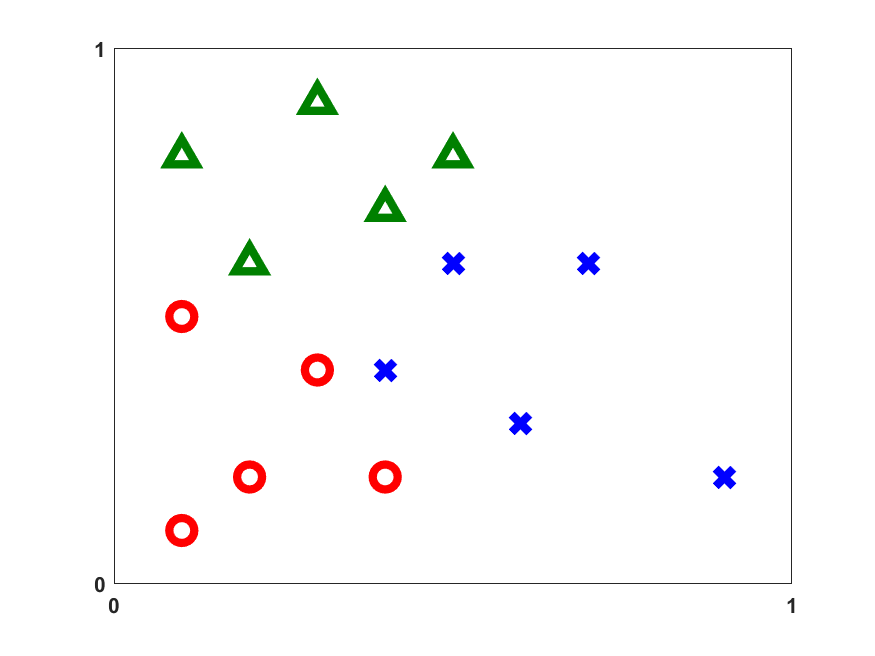
\includegraphics[width=0.5\textwidth]{Figuras/pic_xy.png}
    \caption{Puntos en el plano que marcan las tres categorías}
\end{figure}

De este modo, nuestra red neuronal recibirá como entrada un punto del plano, y nos dirá a qué categoría pertenece, devolviendo $(1,0,0)^T$ si es de la categoría azul, $(0,1,0)^T$ si es de la categoría roja y $(0,0,1)^T$ si es de la categoría amarilla.

Lo siguiente que queremos hacer será entrenar la red neuronal, es decir, ajustar los pesos y sesgos de la red neuronal para que la salida se acerque lo máximo posible a la salida deseada. Es decir, que cuando se introduzca un punto de un tipo concreto, la salida lo asigne a la categoría adecuada. 

Designamos a $y(x)$ como la salida deseada de nuestra red neuronal, y a $F(x)$ como la salida real. Así, el error vendrá dado en función de los pesos y sesgos de la siguiente forma
\begin{equation*}
    \mathcal{L}(W^{[2]},W^{[3]},W^{[4]},b^{[2]},b^{[3]},b^{[4]})=\frac{1}{2}\sum_{x\in X}\|y(x)-F(x)\|^2,
\end{equation*}
donde $X$ es el conjunto de puntos que tenemos para entrenar la red neuronal, en nuestro caso, serán 15. Esta función es conocida como función de coste.

Así, lo que queremos hacer es minimizar esta función, es decir, encontrar los pesos que minimicen la función $\mathcal{L}$. Para ello, se utilizan algoritmos de optimización, como el descenso del gradiente. Este proceso es conocido como el entrenamiento de la red neuronal. Si se logra con éxito, la red neuronal será capaz de clasificar correctamente los puntos en el plano. En este caso concreto, al entrenar la red neuronal, se obtiene la clasificación de la Figura \ref{fig:ClasificacionFinal}, en la que simplemente hemos aplicado nuestra función para cada punto del plano y lo hemos sombreado de acuerdo a la clasificación que se le ha dado.

\begin{figure}
    \centering
    \label{fig:ClasificacionFinal}
    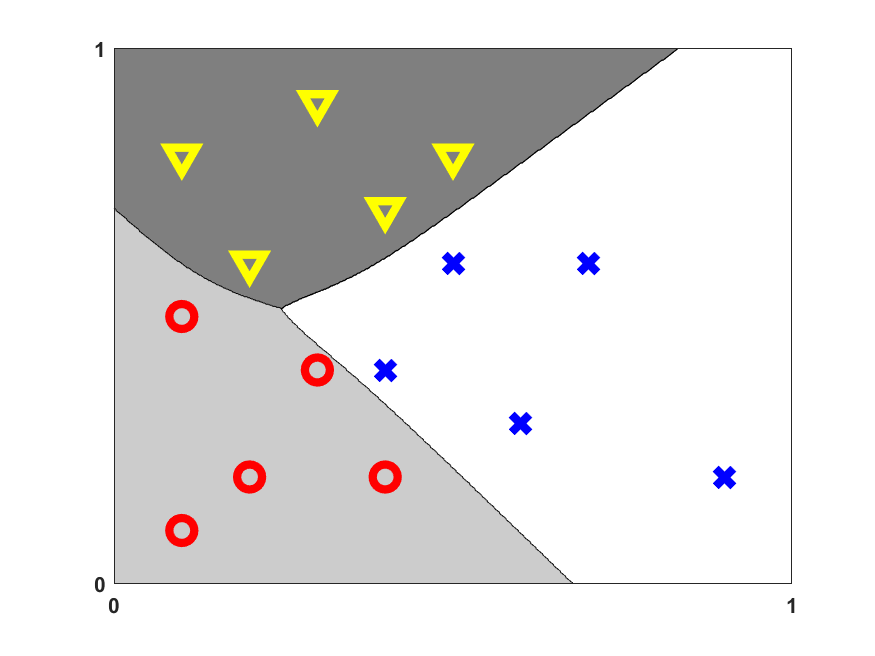
\includegraphics[width=0.5\textwidth]{Figuras/classifier_back.png}
    \caption{Puntos en el plano que marcan las tres categorías}
\end{figure}

Más adelante entenderemos con más detalle como es este proceso de entrenamiento.

\subsection{Comentarios sobre la función sigmoide}\label{subsec:Sigmoide}
Como hemos visto con el ejemplo anterior, las redes neuronales se pueden utilizar para generar funciones. A su vez, estas funciones se utilizan para resolver problemas de forma aproximada. En el ejemplo de la Figura \ref{fig:RedNeuronal}, la función red neuronal clasifica cualquier parte del plano en una de las tres categorías sombreadas a partir del entrenamiento. Dicho entrenamiento fija los valores de los pesos y sesgos, y por tanto define la función red neuronal (en el ejemplo define la función \eqref{eq:RedNeuronal}).

Como las redes neuronales se utilizan para aproximar problemas de tipos muy distintos, una de las características deseables es que sean  capaces de aproximar el conjunto de funciones "mayor posible".

Para poder lograr este objetivo, se necesitan las funciones de activación. Como ejercicio, supongamos que en nuestra ecuación \eqref{eq:RedNeuronal} en lugar de utilizar la función sigmoide, no utilizamos ninguna función de activación, es decir, que nuestra red neuronal es simplemente una composición de funciones lineales. En este caso, nuestra red tendría la siguiente forma

\begin{equation*}
    F(x)=W^{[4]}(W^{[3]}(W^{[2]}x+b^{[2]})+b^{[3]})+b^{[4]}\in\mathbb{R}^3.
\end{equation*}

Claramente, una función lineal definida de forma global puede estar muy lejos de aproximar bien funciones generales. De este modo, parece por tanto razonable utilizar funciones de activación no lineales. La función sigmoide es una de las más utilizadas, pero existen otras como la función tangente hiperbólica o la función ReLU. En este trabajo, nos centraremos en la función sigmoide, que se define como
\begin{equation*}
    \sigma(x)=\frac{1}{1+e^{-x}}.
\end{equation*}

Esta función tiene la ventaja de que su derivada es fácil de calcular, y es precisamente esta derivada la que se utiliza en el algoritmo de entrenamiento de la red neuronal.

Un resultado relevante para justificar el uso de funciones de activación no lineales es el siguiente propuesto por Pinkus \cite[Theorem 3.1]{pinkus1999approximation}. Este resultado es para redes neuronales de una sola capa.

\begin{teor}[Pinkus]
    Sea $\sigma\in C(\mathbb{R})$ y sea $\mathcal{M}(\sigma) = \text{span}\{\sigma(w\cdot x + b): b \in \mathbb{R}, w \in \mathbb{R}^n\}$, se cumple que
    
    Para cualquier $f \in C(\mathbb{R}^n)$, cualquier conjunto compacto $K\in \mathbb{R}^n$ y cualquier $\epsilon > 0$, existe una función $g\in \mathcal{M}(\sigma)$ tal que $\max_{x\in K}|f(x)-g(x)|<\epsilon$ si y solo si $\sigma$ no es una función polinómica.
\end{teor}
De forma más intuitiva, cualquier función $f \in C(\mathbb{R}^n)$, se puede aproximar tan bien como se quiera con una red neuronal de una sola capa si y solo si la función de activación no es polinómica.

Este resultado nos aporta una intuición de por qué las funciones de activación no lineales son necesarias para aproximar funciones de forma general pues, de no ser funciones no lineales, habría muchas funciones que no podríamos aproximar. 

\section{Conceptos preliminares sobre las ecuaciones en derivadas parciales} \label{sec:EDPs}

En este trabajo nos vamos a centrar en las ecuaciones en derivadas parciales elípticas, definidas con la siguiente forma general.

\begin{mdframed}
\begin{defin}\label{def:EDP_eliptica}
    Dado un conjunto $\Omega$, acotado y abierto en $\mathbb{R}^n$, decimos que una ecuación en derivadas parciales es elíptica si es de la siguiente forma:
    \begin{equation}\label{eq:EDP_eliptica}
        -\sum_{i,j=1}^{n} \frac{\partial}{\partial x_j}\left( a_{ij}(x)\frac{\partial u}{\partial x_i}\right) + \sum_{i=1}^{n} b_i(x)\frac{\partial u}{\partial x_i} + c(x)u = f(x), \qquad x\in\Omega.
    \end{equation}
    Donde los coeficientes $a_{ij}(x)$, $b_i(x)$, $c(x)$ y $f$ son funciones que satisfacen las siguientes condiciones
    \begin{align}
        a_{ij} \in C^1(\overline{\Omega}),& \qquad i,j = 1, \dots ,n \label{eq:condiciones_EDP_eliptica_a} \\
        b_i, c \in C(\overline{\Omega}),& \qquad i = 1, \dots ,n \\
        c \in C(\overline{\Omega}),& \\
        f\in C(\overline{\Omega})&\label{eq:condiciones_EDP_eliptica_f}
    \end{align}
    y además cumple la condición de elipticidad uniforme, es decir
    \begin{equation}\label{eq:condiciones_EDP_eliptica_elipticidad_uniforme}
        \sum_{i,j=1}^n a_{ij}(x) \xi_i \xi_j \geq c_0 \sum_{i=1}^n \xi_i^2, \quad \forall \xi = (\xi_1, \ldots, \xi_n) \in \mathbb{R}^n, \quad x \in \overline{\Omega}.
    \end{equation}
\end{defin}
\end{mdframed}

Concretamente, a lo largo del trabajo, nos centraremos en problemas de condición de frontera de Dirichlet, es decir, problemas en los que se cumple que
\begin{equation}
    u(x) = g(x), \qquad \forall x\in\partial\Omega.
\end{equation}

En la formulación que hemos dado de las ecuaciones en derivadas parciales elípticas, nos estábamos refiriendo a su formulación en forma fuerte. No obstante, en muchos casos, no es posible encontrar una solución en forma fuerte, es decir, una función que cumpla la ecuación en todo el dominio y que además cumpla las condiciones de frontera. En estos casos, se recurre a la  formulación débil de la ecuación, que permite encontrar una solución en un espacio de funciones más amplio. Para entender la formulación débil de una ecuación en derivadas parciales, es necesario introducir el concepto de derivada débil.

\begin{mdframed}
    \begin{defin}
        Supongamos que $u$ es una función integrables localmente definida en $\Omega$. Supongamos que tamibén existe una función $w_\alpha$, integrable localmente en $\Omega$, tal que
        \begin{equation*}
            \int_\Omega w_\alpha(x)v(x) \, dx = \int_\Omega u(x)D^\alpha v(x) \, dx, \qquad \forall v \in C_0^\infty(\Omega),
        \end{equation*}
        entonces decimos que $w_\alpha$ es una derivada débil de $u$ de orden $|\alpha| = \alpha_1 + \cdots + \alpha_n$ y escribimos $w_\alpha = D^\alpha u$.
    \end{defin}
\end{mdframed}
\colorbox{yellow}{HAY QUE DEFINIR EL OPERADOR D??}
También es necesario definir el espacio de Sobolev $H^1(\Omega)$.
\begin{mdframed}
\begin{defin}
    Sea $\Omega$ un conjunto abierto de $\mathbb{R}^n$. Definimos el espacio de Sobolev $H^1(\Omega)$ como el conjunto de funciones en el siguiente conjunto
    \begin{equation}
        H^1(\Omega)=\{u\in L^2(\Omega): \frac{\partial u}{\partial x_i}\in L^2(\Omega), \, i=1,\dots,n\}.
    \end{equation}
    En este espacio, se define la siguiente norma
    \begin{equation}
        \|u\|_{H^1(\Omega)}=\left(\|u\|^2_{L^2(\Omega)} + \sum_{i=1}^{n}\left\|\frac{\partial u}{\partial x_i}\right\|^2_{L^2(\Omega)}\right)^{1/2}.
    \end{equation}
    En ambas definiciones las derivadas parciales se entienden en sentido débil.
\end{defin}
\end{mdframed}
    
Definimos demás el espacio $H_0^1(\Omega)$. Este espacio es el cierre de las funciones de $C_0^\infty(\Omega)$ en la norma de $H^1(\Omega)$. Es decir, $H_0^1(\Omega)$ es el conjunto de funciones $u\in H^1(\Omega)$ que se obtienen como límite en $H^1(\Omega)$ de una serie de funciones $\{u_m\}_{m=1}^\infty$ todas ellas en $C_0^\infty(\Omega)$. De este modo, si $\partial\Omega$ es suficientemente regular, $H_0^1(\Omega)$ es el siguiente conjunto:
\begin{equation}
    H_0^1(\Omega)=\{u\in H^1(\Omega): u=0 \text{ en } \partial\Omega\}.
\end{equation}

Con esto, podemos definir la solución débil de una ecuación en derivadas parciales elíptica de la siguiente forma.
\begin{mdframed}
\begin{defin}\label{def:SolucionDebil}
    Dadas las funciones $a_{ij} \in L^\infty(\Omega), \, i,j = 1,\dots, n, \, b_i \in L^\infty(\Omega), \\i= 1, \dots, n, \, c\in L^\infty(\Omega)$, y la función $f\in L^2(\Omega)$. Decimos que la función $u\in H^1_0(\Omega)$ es una solución débil de la ecuación \eqref{eq:EDP_eliptica} con condición de contorno Dirichlet homogénea, es decir, $g(x)=0$ si se cumple que, 
    \begin{equation}\label{eq:SolucionDebil}
        \begin{aligned}
            \sum_{i,j=1}^{n} \int_\Omega a_{ij}(x) \frac{\partial u}{\partial x_i} \frac{\partial \varphi}{\partial x_j}\,dx + \sum_{i=1}^{n} \int_\Omega b_i(x)\frac{\partial u}{\partial x_i} \varphi \,dx  \\+ \int_\Omega c(x)u \varphi \,dx = \int_\Omega f(x)\varphi(x) dx, \qquad \forall \varphi \in H^1_0(\Omega),
        \end{aligned}
    \end{equation}
    donde toas las derivadas parciales en la ecuación \eqref{eq:SolucionDebil} se entienden en sentido débil.
\end{defin}
\end{mdframed}

Si $u $ es una solución clásica de \eqref{eq:EDP_eliptica}, entonces también es una solución débil de \eqref{eq:SolucionDebil}. Sin embargo, lo contrario no es cierto: una solución débil puede no ser lo suficientemente regular para ser una solución clásica. En particular, se demostrará que la ecuación \eqref{eq:EDP_eliptica} tiene una solución débil única $u \in H^1_0(\Omega) $, aunque no tenga solución clásica. Antes de analizar este caso específico, se aborda el problema general de la existencia y unicidad de una solución débil. Para simplificar, se introduce a modo de notación la forma bilineal:
\begin{equation}
    \begin{aligned}
        a(u,\varphi) &= \sum_{i,j=1}^{n} \int_\Omega a_{ij}(x) \frac{\partial u}{\partial x_i} \frac{\partial \varphi}{\partial x_j}\,dx + \sum_{i=1}^{n} \int_\Omega b_i(x)\frac{\partial u}{\partial x_i} \varphi \,dx  \\ &+ \int_\Omega c(x)u \varphi \,dx,
    \end{aligned}
\end{equation}
y el funcional lineal,
\begin{equation}
    l(\varphi) = \int_\Omega f(x)\varphi(x) dx.
\end{equation}
De este modo, nuestro problema elíptico en forma débil se puede expresar de la siguiente manera.
\begin{equation}\label{eq:ProblemaDebilFormaBilineal}
    a(u,\varphi) = l(\varphi) \quad \forall \varphi\in H^1_0(\Omega).
\end{equation}

Para demostrar la existencia y unicidad de una solución para esta ecuación, se puede recurrir al teorema de Lax-Milgram. 

\begin{teor}[Lax-Milgram]
    Sea $V$ un espacio de Hilbert con una norma asociada $\|\cdot\|_V$, y sea $a:V\times V\rightarrow\mathbb{R}$ una forma bilineal y $l:V\rightarrow\mathbb{R}$ un funcional lineal. Si se cumplen las siguientes condiciones
    \begin{itemize}
        \item[(a)] $\exists c_0 > 0 \quad \forall v \in V \quad a(v,v) \geq c_0\|v\|^2$,
        \item[(b)] $\exists c_1 > 0 \quad \forall v, w \in V \quad |a(w,v)| \leq c_1\|w\|\|v\|$,
    \end{itemize}
    y sea $l(\cdot)$ un funcional lineal en $V$ tal que:
    \begin{itemize}
        \item[(c)] $\exists c_2 > 0 \quad \forall v \in V \quad |l(v)| \leq c_2\|v\|$.
    \end{itemize}
    entonces, existe una única solución débil $u\in V$ tal que
    \begin{equation*}
        a(u,v) = l(v) \quad \forall v\in V.
    \end{equation*}
\end{teor}
Con este teorema se puede demostrar que una ecuación elíptica con condiciones de contorno Dirichlet homogéneas tiene solución única en $H^1_0(\Omega)$. Para ello se puede aplicar el teorema de Lax-Milgram en el espacio $V=H^1_0(\Omega)$ con la norma $\|\cdot\|_{H^1(\Omega)}$ y las formas bilineal y lineal $a$ y $l$ definidas anteriormente. Para que se cumplan las condiciones $(a,b,c)$ del teorema, además de la condición de elipticidad uniforme es necesario requerir que
\begin{equation}\label{eq:condiciones_LaxMilgram_extra}
    c(x) - \frac{1}{2} \sum_{i=1}^n \frac{\partial b_i}{\partial x_i} \geq 0, \quad x \in \overline{\Omega}.
\end{equation}

\colorbox{yellow}{DEJO LA DEMOSTRACIÓN ESCRITA POR SI LA QUEREMOS PONER}

De esta manera, se demuestran las condiciones (a), (b) y (c) del teorema de Lax-Milgram como sigue.
\begin{dem}
    Empezamos por la condición (c).
    \begin{itemize}
        \item[(c)] La aplicación $v \mapsto l(v)$ es lineal: de hecho, para cualesquiera $\alpha, \beta \in \mathbb{R}$, 
        \begin{align*}
            l(\alpha v_1 + \beta v_2) &= \int_{\Omega} f(x)(\alpha v_1(x) + \beta v_2(x)) \, dx \\
            &= \alpha \int_{\Omega} f(x)v_1(x) \, dx + \beta \int_{\Omega} f(x)v_2(x) \, dx \\
            &= \alpha l(v_1) + \beta l(v_2), \quad v_1, v_2 \in H_0^1(\Omega).
        \end{align*}
        Por lo tanto, $l(\cdot)$ es una funcional lineal en $H_0^1(\Omega)$. Además, por la desigualdad de Cauchy-Schwarz,
        \begin{align*}
            |l(v)| &= \left| \int_{\Omega} f(x)v(x) \, dx \right| \leq \left(\int_{\Omega} |f(x)|^2 \, dx \right)^{1/2} \left(\int_{\Omega} |v(x)|^2 \, dx \right)^{1/2} \\
            &= \|f\|_{L^2(\Omega)} \|v\|_{L^2(\Omega)} \leq \|f\|_{L^2(\Omega)} \|v\|_{H^1(\Omega)},
        \end{align*}
        para todo $v \in H_0^1(\Omega)$, donde hemos usado la desigualdad obvia $\|v\|_{L^2(\Omega)} \leq \|v\|_{H^1(\Omega)}$. Tomando $c_2 = \|f\|_{L^2(\Omega)}$, obtenemos la cota requerida.
        \item [(b)] A continuación, verificamos (b). Para cualquier $w \in H_0^1(\Omega)$, la aplicación $v \mapsto a(v, w)$ es lineal. De manera similar, para cualquier $v \in H_0^1(\Omega)$, la aplicación $w \mapsto a(v, w)$ es lineal. Por lo tanto, $a(\cdot, \cdot)$ es una funcional bilineal en $H_0^1(\Omega) \times H_0^1(\Omega)$. Aplicando la desigualdad de Cauchy-Schwarz, deducimos que
        \begin{align*}
            |a(w, v)| \leq & \sum_{i, j = 1}^n \max_{x \in \overline{\Omega}} |a_{ij}(x)|\left| \int_{\Omega}  \frac{\partial w}{\partial x_i} \frac{\partial v}{\partial x_j} dx \right|  \\
            &+ \sum_{i = 1}^n \max_{x \in \overline{\Omega}} |b_i(x)| \left|  \int_{\Omega} \frac{\partial w}{\partial x_i} v dx \right| \\
            &+ \max_{x \in \overline{\Omega}} |c(x)| \left| \int_{\Omega}  w(x)v(x) dx \right|  \\
            &\leq \hat{c} \Bigg\{
            \left( \sum_{i,j=1}^n \int_\Omega \left| \frac{\partial w}{\partial x_i} \right|^2 dx \right)^{1/2}
            \left( \int_\Omega \left| \frac{\partial v}{\partial x_j} \right|^2 dx \right)^{1/2}\\
            &+ \sum_{i=1}^n \left( \int_\Omega \left| \frac{\partial w}{\partial x_i} \right|^2 dx \right)^{1/2}
            \left( \int_\Omega |v|^2 dx \right)^{1/2} \\
            &+ \left( \int_\Omega |w|^2 dx \right)^{1/2}
            \left( \int_\Omega |v|^2 dx \right)^{1/2}
            \Bigg\}\\
            &\leq \hat{c} \Bigg\{
            \left( \int_\Omega |w|^2 dx \right)^{1/2}
            + \sum_{i=1}^n \left( \int_\Omega \left| \frac{\partial w}{\partial x_i} \right|^2 dx \right)^{1/2}
            \Bigg\} \\
            &\times
            \Bigg\{
            \left( \int_\Omega |v|^2 dx \right)^{1/2}
            + \sum_{j=1}^n \left( \int_\Omega \left| \frac{\partial v}{\partial x_j} \right|^2 dx \right)^{1/2}
            \Bigg\}.
        \end{align*}
        donde
        \begin{align*}
            \hat{c} = \max \Bigg\{ \max_{1 \leq i,j \leq n} \max_{x \in \overline{\Omega}} |a_{ij}(x)|, \max_{1 \leq i \leq n} \max_{x \in \overline{\Omega}} |b_i(x)|, \max_{x \in \overline{\Omega}} |c(x)| \Bigg\}.
        \end{align*}

        Si acotamos aún más el lado derecho de la última desigualdad, deducimos que
        \begin{align*}
            |a(w, v)| \leq 2\hat{c} \Bigg\{ \left(\int_{\Omega} |w|^2 dx + \sum_{i=1}^n \int_{\Omega} \left| \frac{\partial w}{\partial x_i} \right|^2 dx \right)^{1/2} \\
            \times \left(\int_{\Omega} |v|^2 dx + \sum_{j=1}^n \int_{\Omega} \left| \frac{\partial v}{\partial x_j} \right|^2 dx \right)^{1/2} \Bigg\},
        \end{align*}
        por lo que, tomando $c_1 = 2\hat{c}$, obtenemos la desigualdad de (b).
        \item[(a)] Por último, demostramos la condición (a). Aquí utilizaremos la condición extra requerida en \eqref{eq:condiciones_LaxMilgram_extra} y la condición de elipticidad uniforme \eqref{eq:condiciones_EDP_eliptica_elipticidad_uniforme}. Usando  \eqref{eq:condiciones_EDP_eliptica_elipticidad_uniforme} y la desigualdad de Cauchy-Schwarz,
        \begin{align*}
        a(v, v) &\geq \tilde{c} |v|^2_{H^1(\Omega)} - 
        \left( \sum_{i=1}^{n} \|b_i\|^2_{L_{\infty}(\Omega)} \right)^{1/2} 
        |v|_{H^1(\Omega)} \|v\|_{L_2(\Omega)} 
        + \int_{\Omega} c(x) |v(x)|^2 dx \\
        &\geq \frac{1}{2} \tilde{c} |v|^2_{H^1(\Omega)} 
        + \int_{\Omega} \left( c(x) - \frac{2}{\tilde{c}} \sum_{i=1}^{n} \|b_i\|^2_{L_{\infty}(\Omega)} \right) |v(x)|^2 dx.
        \end{align*}
        Asumiendo que 
        \begin{align*}
        c(x) - \frac{2}{\tilde{c}} \sum_{i=1}^{n} \|b_i\|^2_{L_{\infty}(\Omega)} \geq 0,
        \end{align*}
        llegamos a la desigualdad 
        \begin{align}\label{eq:resultado_aplicar_condicion_a}
        a(v, v) \geq \frac{1}{2} \tilde{c} \sum_{i=1}^{n} \int_{\Omega} \left| \frac{\partial v}{\partial x_i} \right|^2 dx.
        \end{align}
        Mediante la desigualdad de Poincaré-Friedrichs, el lado derecho puede acotarse aún más para obtener
        \begin{align}\label{eq:desigualdad_Poincaré_Friedrichs_demo_a}
        a(v, v) \geq \frac{\tilde{c}}{c_{\star}} \int_{\Omega} |v|^2 dx.
        \end{align}
        Juntando \eqref{eq:resultado_aplicar_condicion_a} y \eqref{eq:desigualdad_Poincaré_Friedrichs_demo_a}, obtenemos
        \begin{align}
        a(v, v) \geq c_0 \left( \int_{\Omega} |v|^2 dx + \sum_{i=1}^{n} \int_{\Omega} \left| \frac{\partial v}{\partial x_i} \right|^2 dx \right),
        \end{align}
        donde $c_0 = \tilde{c}/(1 + c_{\star})$, y por queda demostrado (a).
    \end{itemize}
    Se comprueban así las condiciones (a), (b) y (c) del teorema de Lax-Milgram y concluimos que existe una única solución débil en $H^1_0(\Omega)$ para la ecuación \eqref{eq:ProblemaDebilFormaBilineal}.
\end{dem}

\section{Métodos numéricos tradicionales: el método de los elementos finitos}\label{sc:FEM}

El método de los elementos finitos (FEM por su siglas en inglés) es una técnica numérica para resolver ecuaciones en derivadas parciales. Este método es ampliamente utilizado en ingeniería y ciencias aplicadas porque permite aproximar soluciones en dominios complejos.

Para un problema elíptico con condiciones de contorno Dirichlet homogéneas, se parte de la ecuación en su formulación débil. Como hemos visto en el apartado anterior, este problema se puede formular de forma simplificada como encontrar $u\in H_0^1(\Omega)$ tal que
\begin{equation*}
    a(u,\varphi) = l(\varphi) \quad \forall \varphi\in  H_0^1(\Omega).
\end{equation*}

Por lo visto en la sección \ref{sec:EDPs}, esta ecuación tiene solución única en $H_0^1(\Omega)$ si se cumple la condición de \eqref{eq:condiciones_LaxMilgram_extra}. De este modo, para que la formulación del problema sea válida, asumiremos que se cumple esta condición.

Lo siguiente que se hace es dividir el dominio $\Omega$ en un conjunto de subdominios más pequeños, llamados elementos finitos. Por ejemplo, si estamos trabajando con un problema de una dimensión, con $\Omega =(0,1)$, dividimos $\overline{\Omega} = [0,1]$ en $N$ subintervalos $[x_i,x_{i+1}], \, i = 1, \dots, N-1$, con $x_i = ih$, obteniendo la división de la Figura \ref{fig:DivisionOmega}.

\begin{figure}
    \centering
    \begin{tikzpicture}
        \draw[thick] (0,0) -- (12,0); % Adjusted length of the line
        \foreach \x in {0,2,4,6,8,10,12} % Adjusted positions of the ticks
        \draw (\x cm,3pt) -- (\x cm,-3pt);
        \draw (0,0) node[below=3pt] {$x_0 = 0$};
        \draw (2,0) node[below=3pt] {$x_1$};
        \draw (4,0) node[below=3pt] {$x_2$};
        \draw (6,0) node[below=3pt] {$x_3$};
        \draw (8,0) node[below=3pt] {$\dots$};
        \draw (10,0) node[below=3pt] {$x_{N-1}$};
        \draw (12,0) node[below=3pt] {$x_{N}=1$};
    \end{tikzpicture}
    \caption{División de $\Omega = (0,1)$ en $N$ elementos finitos}
    \label{fig:DivisionOmega}
\end{figure}

A esta subdivision, se le asocia una base de polinomios a trozos. Remplazando así el subespacio de funciones que habíamos llamado $H_0^1(\Omega)$ por un subespacio de dimensión finita $V_h$ formado por polinomios a trozos  de grado fijo. Siguiendo nuestro ejemplo de antes, la base de polinomios que vamos a utilizar será la de los polinomios como los vistos en la Figura \ref{fig:BasePolinomios}. Definidos de la siguiente forma.
\begin{equation*}
    \phi_i(x) = \begin{cases}
        \frac{x-x_{i-1}}{x_i-x_{i-1}}, & \text{si } x\in[x_{i-1},x_i],\\
        \frac{x_{i+1}-x}{x_{i+1}-x_i}, & \text{si } x\in[x_i,x_{i+1}],\\
        0, & \text{en otro caso}.
    \end{cases} 
\end{equation*}

\begin{figure}
    \centering
    \begin{tikzpicture}[scale=0.5]
        \draw[thick] (0,0) -- (12,0); % Adjusted length of the line
        \draw (6 cm,100pt) -- (6 cm,-5pt);
        \draw (1 cm,5pt) -- (1 cm,-5pt);
        \draw (11 cm,5pt) -- (11 cm,-5pt);
        \draw[thick] (1,0) -- (6,100pt) -- (11,0);
        \draw (1,0) node[below=3pt] {$x_{i-1}$};
        \draw (6,0) node[below=3pt] {$x_i$};
        \draw (11,0) node[below=3pt] {$x_{i+1}$};
    \end{tikzpicture}
    \caption{Polinomio $\phi_i$}
    \label{fig:BasePolinomios}
\end{figure}

En este ejemplo, nuestro espacio de funciones será $V_h = \text{span}\{\phi_1,\dots,\phi_{N-1}\}$, donde $N$ es el número de elementos finitos en los que hemos dividido el dominio. Con esta definición es claro que todos los $\phi_i\in H_0^1(\Omega)$ pues son funciones derivable en sentido débil que valen $0$ en la frontera de $\Omega =(0,1)$. De este modo, al buscar soluciones en este nuevo espacio de funciones, nuestra ecuación diferencial elíptica se convertiría en encontrar $u_h\in V_h$ tal que
\begin{equation*}
    a(u_h,v_h) = l(v_h) \quad \forall v_h\in V_h,
\end{equation*}
Nótese que las condiciones de contorno van implícitas en la definición de $V_h$ pues todos los $\phi_i\in H_0^1(\Omega)$. 

Con todo, de forma intuitiva, lo que se hace es que en vez de buscar una solución en un espacio de funciones de dimensión infinita, como es $H_0^1(\Omega)$, se busca una solución en un espacio de funciones de dimensión finita, como es $V_h$. Para poder hacer eso, que nos simplifica mucho el problema, lo que hemos hecho es que nuestro dominio, lo hemos dividido en subdominios más pequeños a partir de los cuales hemos construido nuestro nuevo espacio de funciones. 

Ahora, encontrar una solución se convierte en encontrar los coeficientes en la base de polinomios a trozos, es decir, los $U_i$ en la siguiente ecuación
\begin{equation}
    u_h = \sum_{i=1}^{N-1} U_i\phi_i.
\end{equation}
Por tanto, resolver la ecuación diferencial se convierte en encontrar $U=(U_1,\dots, U_{N-1}) \in \mathbb{R}^{N-1}$ que cumplen:
\begin{equation}
    \sum_{i=1}^{N-1} a\left( \phi_i,\phi_j\right)U_i = l(\phi_j) \quad \forall j = 1,\dots,N-1.
\end{equation}

Esto se traduce en un sistema lineal de la forma $AU = b$, donde $A$ es la matriz de rigidez (con entradas $A_{ij}=a\left( \phi_i,\phi_j\right)$), y $b$ es el vector de términos fuente (con entradas $b_j = l(\phi_j)$). A este nuevo sistema lineal se le pueden aplicar métodos numéricos tradicionales para resolverlo, como la factorización LU, encontrando así los coeficientes $U$ que nos dan $u_h$, la aproximación de $u$.

Este proceso se puede generalizar a problemas en más dimensiones, donde se dividen los dominios en elementos finitos de mayor dimensión, y se construye una base de polinomios a trozos en cada uno de estos elementos. Por ejemplo, en dos dimensiones, un elemento finito sería un triángulo, y la base de polinomios a trozos sería una base de funciones que valen $0$ en los bordes del triángulo y que son lineales en cada uno de los lados del triángulo.

\begin{mdframed}  
\begin{exmp}
    Veamos ahora un ejemplo concreto de la aplicación del FEM a través de la ecuación de Poisson en dos dimensiones. El objetivo es encontrar un campo escalar $ u $ sobre un dominio $\Omega \subset \mathbb{R}^n$ que satisfaga:
    \begin{equation}
    \begin{aligned}
    - \nabla^2 u &= f \quad \text{en} \ \Omega, \\
    u &= 0 \quad \text{en} \ \partial\Omega, \\
    \end{aligned}
    \end{equation}
    donde $ f $ es un término fuente y la condición de contorno es de Dirichlet homogénea. Para encontrar una solución, construimos la forma débil de la ecuación. Para ello, tomamos $v\in H_0^1(\Omega)$ y multiplicamos ambos lados por $v$ e integramos sobre $\Omega$.
    \begin{equation*}
        -\int_{\Omega} (\nabla^2 u) v \, dx = \int_{\Omega} f v \, dx.
    \end{equation*}
    Utilizando la identidad $div(v\nabla u) = (\nabla u)(\nabla v) + v \nabla^2u$ obtenemos:
    \begin{equation*}
    \int_{\Omega} \nabla u \nabla v - \int_{\Omega} div(v \nabla u) = \int_{\Omega} f v
    \end{equation*}
    Por el teorema de Green, podemos escribir (si \(\partial \Omega\) es suficientemente regular):
    \begin{equation*}
    \int_{\Omega} \nabla u \nabla v - \int_{\partial \Omega} (v \nabla u) \cdot \mathbf{n} \, dS = \int_{\Omega} f v
    \end{equation*}
    Finalmente, dado que \(v = 0\) en \(\partial \Omega\), concluimos:
    \begin{equation*}
    \int_{\Omega} \nabla u \nabla v = \int_{\Omega} f v
    \end{equation*}
    La forma fuerte del problema se convierte en: 
    \begin{equation}\label{eq:forma_debil_poisson}
    a(u, v) = l(v) \quad \forall \ v \in H_0^1(\Omega),
    \end{equation}
    donde:
    \begin{itemize}
        \item $ a(u, v) = \int_{\Omega} \nabla u \cdot \nabla v \, \text{d}x $
        \item $ l(v) = \int_{\Omega} f v \, dx $
    \end{itemize}
    Para aplicar el FEM, nos interesa encontrar una solución aproximada en un espacio de funciones de dimensión finita. Para ello, dividimos el dominio $\Omega$ en un conjunto de elementos finitos y construimos una base de polinomios a trozos en cada uno de estos elementos. 
    
    Antes de seguir avanzando, para este ejemplo específico, tomaremos un dominio rectangular $\Omega = [0,2] \times [0,1]$ y $f(x, y) = 10 \cdot\exp \left( - \frac{(x - 0.5)^2 + (y - 0.5)^2}{0.02} \right)$. Bajo estas condiciones sabemos que existe una solución única en $H_0^1(\Omega)$ para el problema \eqref{eq:forma_debil_poisson}.

    A continuación, usamos el paquete de python FEniCS para resolver el problema. En el, lo único reseñable es que se define el dominio $\Omega$ y la malla de elementos finitos con el siguiente comando
    \begin{lstlisting}[language=Python]
    msh = mesh.create_rectangle(
        comm=MPI.COMM_WORLD,
        points=((0.0, 0.0), (2.0, 1.0)),
        n=(32, 16),
        cell_type=mesh.CellType.triangle,
    )
    \end{lstlisting}
    y se especifica el tipo de polinomios a trozos que se van a utilizar para la base de funciones, en este caso polinomios de Lagrange de grado 1
    \begin{lstlisting}[language=Python]
        V = FunctionSpace(msh, "Lagrange", 1)
    \end{lstlisting}
    Con esto, obtenemos el resultado que se puede ver en la Figura \ref{fig:poisson}.
    \begin{figure}[H] 
        \centering
        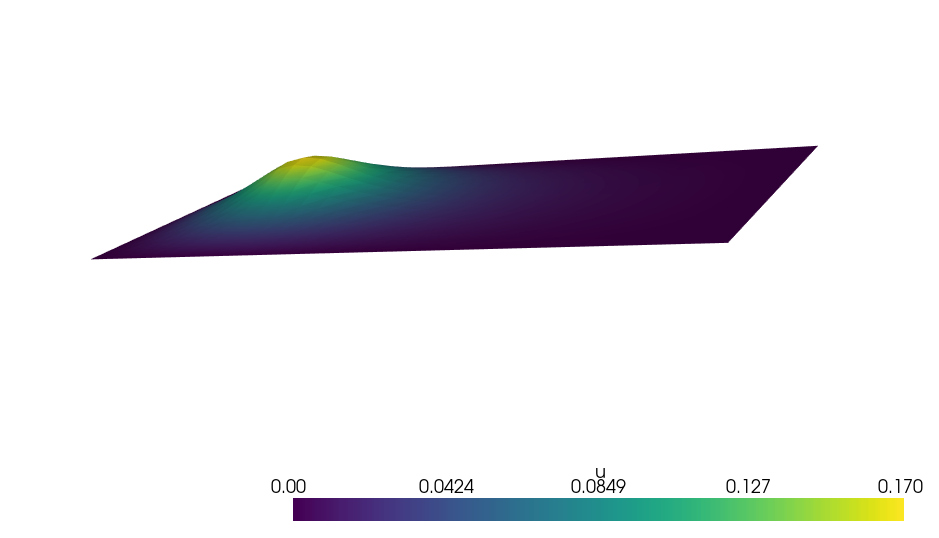
\includegraphics[width=0.5\textwidth]{Figuras/poisson.png}
        \caption{Solución de la ecuación de Poisson}
        \label{fig:poisson}
    \end{figure}
    En el que la malla de elementos finitos utilizada para la aproximación de la solución se puede apreciar en la Figura \ref{fig:poisson_malla}.
    \begin{figure}[H]
        \centering
        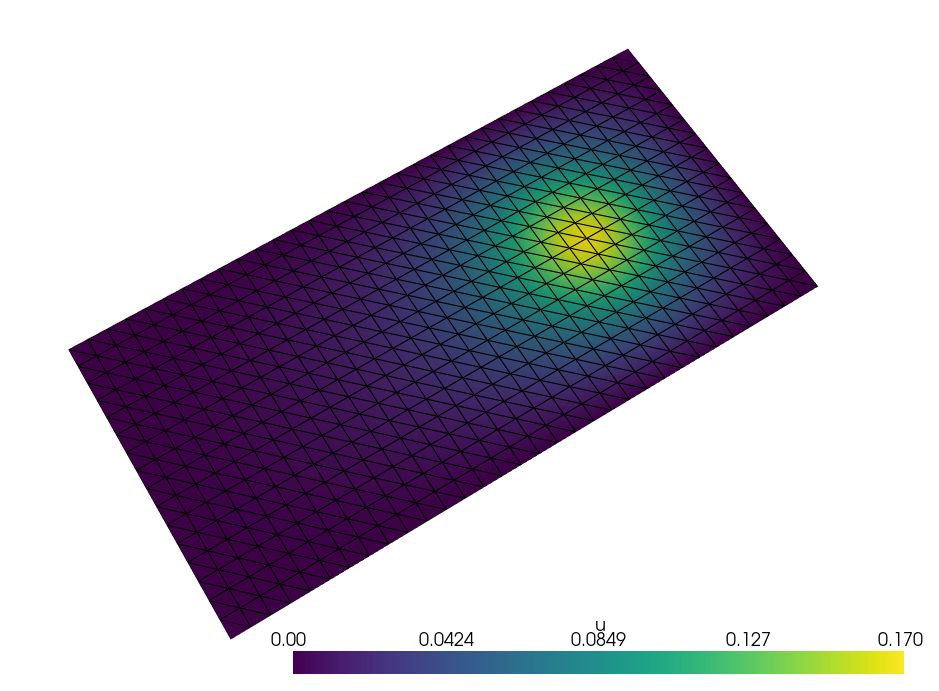
\includegraphics[width=0.5\textwidth]{Figuras/malla_poisson.png}
        \caption{Malla de elementos finitos}
        \label{fig:poisson_malla}
    \end{figure}
\end{exmp}
\end{mdframed}

\chapter{Aproximación de EDPs mediante redes neuronales}\label{chap2}

\section{PINN: Physics-Informed Neural Networks}\label{sec:PINN}
\subsection{Introducción}
Las PINN, o Physics-Informed Neural Networks, son una técnica que combina la resolución de ecuaciones en derivadas parciales con redes neuronales. La idea es que, en vez de resolver la ecuación diferencial directamente o con métodos numéricos tradicionales, se entrena una red neuronal para que aproxime la solución de la ecuación. 

Como habíamos comentado en la Sección \ref{sec:RedesNeuronales}, las redes neuronales son capaces de aproximar cualquier función, por lo que, en teoría, pueden aproximar cualquier solución de una ecuación diferencial. De este modo, las PINN van a aprovechar esto, definiendo la aproximación de nuestra solución ${u}$, como la salida de la función red neuronal $\hat{u}(x;\mathbf{\theta})$,  donde $\theta$ hace referencia a los pesos y sesgos vistos en la Sección \ref{sec:RedesNeuronales}. Así, la función en la Figura \ref{fig:PIN} sería la aproximación de la solución de la ecuación diferencial.
\begin{figure}[htbp]
    \centering
    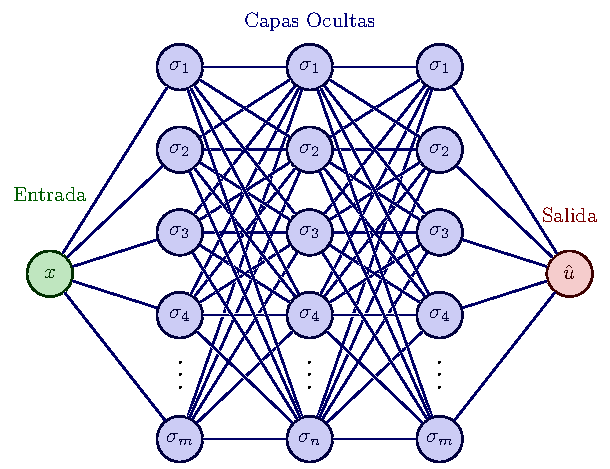
\includegraphics[scale=0.6]{Figuras/neural_network_improved.pdf}
    \caption{Esquema de una PINN}
    \label{fig:PIN}
\end{figure}

\subsection{Formulación de las PINN}
Consideramos una EDP de la forma vista en la Sección \ref{sec:EDPs}, es decir, una EDP elíptica sujeta a condiciones de contorno Dirichlet. De modo que la ecuación a resolver es la siguiente: 
\begin{equation} 
    \begin{cases} -\sum_{i,j=1}^{n} \frac{\partial}{\partial x_j}\left( a_{ij}(\mathbf{x})\frac{\partial u}{\partial x_i}\right) + \sum_{i=1}^{n} b_i(\mathbf{x})\frac{\partial u}{\partial x_i} + c(\mathbf{x})u = f(\mathbf{x}), &\qquad \mathbf{x}\in\Omega,\\ u(\mathbf{x}) = g(\mathbf{x}), &\qquad \mathbf{x}\in\partial\Omega. 
    \end{cases} 
\end{equation} 
donde $\Omega \subset \mathbb{R}^n$ es un dominio y las funciones $a_{ij}(\mathbf{x})$, $b_i(\mathbf{x})$, $c(\mathbf{x})$, $f(\mathbf{x})$ y $g(\mathbf{x})$ son conocidas. La incógnita es la función $u: \Omega \to \mathbb{R}$ que satisface la ecuación diferencial y las condiciones de contorno. Para poder construir y ajustar los pesos de una red neuronal que aproxime $u$ es esencial tener una función de coste, es decir, una función que nos indique la calidad de nuestra aproximación. En el caso de las PINN, la función de coste se define como la suma ponderada de dos términos. El primero de ellos garantiza que la función aproximada por la red neuronal satisface la ecuación diferencial en todo el dominio. El segundo término asegura que la aproximación satisface las condiciones de contorno de Dirichlet
\begin{equation} \label{eq:L_PINN}
    \mathcal{L}(\boldsymbol{\theta}; \mathcal{T}) = w_f \mathcal{L}_f(\boldsymbol{\theta}; \mathcal{T}_f) + w_b \mathcal{L}_b(\boldsymbol{\theta}; \mathcal{T}_b),
\end{equation}
donde $w_f$ y $w_b$ son pesos que se ajustan para dar más importancia a un término u otro y
\begin{equation}
    \label{eq:Lf_Lb}
    \begin{split}
        \mathcal{L}_f(\boldsymbol{\theta}; \mathcal{T}_f) &= \frac{1}{|\mathcal{T}_f|} \sum_{\mathbf{x} \in \mathcal{T}_f} || -\sum_{i,j=1}^{n} \frac{\partial}{\partial x_j}\left( a_{ij}(\mathbf{x})\frac{\partial \hat{u}}{\partial x_i}\right) \\ &+ \sum_{i=1}^{n} b_i(\mathbf{x})\frac{\partial \hat{u}}{\partial x_i} + c(\mathbf{x})\hat{u} - f(\mathbf{x}) ||_2^2, \\ 
        \mathcal{L}_b(\boldsymbol{\theta}; \mathcal{T}_b) &= \frac{1}{|\mathcal{T}_b|} \sum_{\mathbf{x} \in \mathcal{T}_b} \left\| \hat{u} (\mathbf{x}) - g(\mathbf{x})\right\|_2^2,
    \end{split}
\end{equation}
    
Estas funciones $\mathcal{L}_f$ y $\mathcal{L}_b$ se obtienen a través de una regla de cuadratura. Con las PINN nosotros queremos encontrar una función $\hat{u}$ que minimice el residuo en $\Omega$ y que cumpla las condiciones de contorno en $\partial\Omega$. Para ello, lo que queremos es la $\hat{u}$ que haga que las siguientes expresiones sean mínimas:
\begin{align*}
    &\int_{\mathbf{x} \in \Omega} \left\| -\sum_{i,j=1}^{n} \frac{\partial}{\partial x_j}\left( a_{ij}(\mathbf{x})\frac{\partial \hat{u}}{\partial x_i}\right) + \sum_{i=1}^{n} b_i(\mathbf{x})\frac{\partial \hat{u}}{\partial x_i} + c(\mathbf{x})\hat{u} - f(\mathbf{x}) \right\|_2^2, \\ 
    &\int_{\mathbf{x} \in \partial\Omega} \left\| \hat{u} (\mathbf{x}) - g(\mathbf{x})\right\|_2^2,
\end{align*}
Para poder computar estas integrales, se utiliza una regla de cuadratura que las aproxime mediante sumas ponderadas de los valores de las funciones en un conjunto discreto de puntos. En este contexto, los puntos de evaluación se denominan puntos de colocación o collocation points. Para la primera expresión, los puntos de colocación que se usarán los denominaremos $\mathcal{T}_f$, mientras que para la segunda los denominaremos $\mathcal{T}_b$. 

De este modo, para obtener la ecuación \eqref{eq:Lf_Lb} se usará una cuadratura de Gauss con pesos constantes $\frac{w_f}{|\mathcal{T}_f|}$ y $\frac{w_b}{|\mathcal{T}_b|}$ respectivamente. 

Existe mucha literatura sobre como tomar los puntos de colocación pues, al igual que en FEM la malla impacta el resultado, en las PINN, el conjunto $\mathcal{T}$ determina como de bien nuestra red neuronal se ajusta a la solución \cite{münzer2022curriculumtrainingbasedstrategydistributingcollocation}\cite{aikawa2024improving}\cite{matsubara2023goodlatticetrainingphysicsinformed}\cite{subramanian2022adaptiveselfsupervisionalgorithmsphysicsinformed}\cite{hou2023enhancing}.  

Es importante destacar que con esta formulación, se impone que el residuo en forma fuerte de la ecuación diferencial sea cero en los puntos de colocación, lo cual, veremos más adelante que puede ser una fuente de errores. 

Dada la función de coste definida y la distribución de los puntos de colocación, el siguiente paso es el entrenamiento. Este re reduce a resolver un problema de optimización: encontrar los parámetros $\theta$ que minimizan la función de coste $\mathcal{L}(\boldsymbol{\theta}; \mathcal{T})$. Para ello, es habitual emplear métodos de optimización basados en gradientes, como Adam o L-BFGS. 

Una ventaja fundamental del uso de redes neuronales en este contexto es la diferenciación automática, una técnica numérica muy potente que facilita la obtención de las derivadas de $\hat{u}$ con respecto a sus entradas de forma exacta y eficiente.
A continuación, vamos a ver dos ejemplos para ver como se aplican las PINN a problemas concretos.

\begin{mdframed}
    \begin{exmp}
        Consideramos la ecuación elíptica unidimensional:
        \begin{equation*}
        -u_{xx} = \pi^2 \sin(\pi x), \quad x \in [-1, 1],
        \end{equation*}
        con las condiciones de contorno de Dirichlet
        \begin{equation*}
        u(-1) = 0, \quad u(1) = 0.
        \end{equation*}
        En esta ecuación la solución exacta es  conocida $ u(x) = \sin(\pi x)$. Para resolver este problema con una PINN, nos asistimos de la librería de python DeepXDE \cite{lu2021deepxde}, la cual tiene implementada la funcionalidad necesaria para entrenar una red neuronal que aproxime EDPs. Así, comenzamos definiendo el intervalo en el que se encuentra el dominio y los puntos de colocación
        
\begin{lstlisting}[language=Python]
    geom = dde.geometry.Interval(-1, 1)
\end{lstlisting}
        definimos la EDP
\begin{lstlisting}[language=Python]
    def pde(x, y):
        dy_xx = dde.grad.hessian(y, x)
        return -dy_xx - np.pi ** 2 * tf.sin(np.pi * x)
\end{lstlisting}
    indicamos las condiciones de contorno de Dirichlet
\begin{lstlisting}[language=Python]
    bc = dde.icbc.DirichletBC(geom, func, boundary)
\end{lstlisting}
y, con todo, se define el problema de EDPs
\begin{lstlisting}[language=Python]
   data = dde.data.PDE(geom, pde, bc, 16, 2, solution=func, num_test=100)
\end{lstlisting}
    Gracias a la librería DeepXDE, podemos entrenar la red neuronal con el siguiente código
\begin{lstlisting}[language=Python]
Losshistory, train_state = model.train(
    iterations=10000, callbacks=[checkpointer, movie]
)
\end{lstlisting}
    Por detrás, esta se encargará de definir la función de coste asociada, que en este caso será
    \begin{equation*} 
        \mathcal{L}(\boldsymbol{\theta}; \mathcal{T}) = w_f \mathcal{L}_f(\boldsymbol{\theta}; \mathcal{T}_f) + w_b \mathcal{L}_b(\boldsymbol{\theta}; \mathcal{T}_b),
    \end{equation*}
    donde
    \begin{align*}
        \mathcal{L}_f(\boldsymbol{\theta}; \mathcal{T}_f) &= \frac{1}{|\mathcal{T}_f|} \sum_{\mathbf{x} \in \mathcal{T}_f} | \hat{u}_{xx} +\pi^2 \sin(\pi x)|^2, \\ 
        \mathcal{L}_b(\boldsymbol{\theta}; \mathcal{T}_b) &= \frac{1}{|\mathcal{T}_b|} \sum_{\mathbf{x} \in \mathcal{T}_b} | \hat{u} (\mathbf{x})|^2,
    \end{align*}
    por los argumentos con los que se han inicializado las funciones, $\mathcal{T}_f$ serán 16 puntos aleatorios en el intervalo $[-1,1]$ y $\mathcal{T}_b = \{0,1\}$ . Con todo, el resultado de ejecutar este código será el de la Figura \ref{fig:poisson_PINN}.

    \begin{figure}[H] 
        \centering
        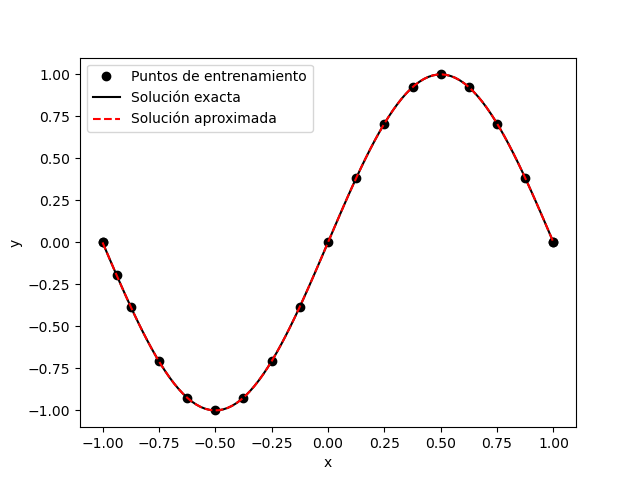
\includegraphics[width=0.6\textwidth]{Figuras/Poisson.png}
        \caption{Solución de la ecuación de Poisson}
        \label{fig:poisson_PINN}
    \end{figure}
\end{exmp}
\end{mdframed}

No obstante, las PINN pueden presentar errores elevados incluso en sistemas relativamente simples. A continuación, vemos uno de los ejemplos que presentan en Luo et al. en \cite{luo2023residualminimizationpdesfailure} en los que las PINN fallan.

\begin{mdframed}
    \begin{exmp}
        La ecuación considerada es unidimensional y se expresa como
        \begin{equation}
            \left\{
            \begin{aligned}
                L u =-D_{x}(AD_{x} u) &=f\quad \text{en}\  \Omega=(-1,1), \\
                u &=0\quad \text{en}\  \partial\Omega=\{-1,1\},
            \end{aligned}
            \right.
        \end{equation}
        donde la función coeficiente $A$ y $f$ son ambas funciones continuas a trozos y se expresan como
        \begin{equation}\label{eq:1dCoeff}
            A(x)=\left\{
            \begin{aligned}
                & \tfrac{1}{2}, & & x\in (-1,0), \\
                &1, & & x\in [0,1),
            \end{aligned}
            \right.\quad 
            f(x)=\left\{
            \begin{aligned}
                & 0, & & x\in (-1,0), \\
                & -2, & & x\in [0,1).
            \end{aligned}
            \right.
        \end{equation}
        Claramente, no existe una solución fuerte. Sin embargo la solución débil $u\in H^1(-1,1)$ para esta ecuación es
        \begin{equation}\label{eq:SolTo1dEq}
            u(x)=
            \left\{
            \begin{aligned}
                & -\tfrac{2}{3}x-\tfrac{2}{3}, & & x\in (-1,0), \\
                & x^2-\tfrac{1}{3}x-\tfrac{2}{3}, & & x\in [0,1).
            \end{aligned}
            \right.
        \end{equation}
        En la serie de experimentos numéricos, utilizamos una red neuronal con la siguiente configuración $1$-$256$-$256$-$256$-$1$.  Así, la función de coste vendrá dada por la siguiente función.
        \begin{equation*} 
            \mathcal{L}(\boldsymbol{\theta}; \mathcal{T}) = w_f \mathcal{L}_f(\boldsymbol{\theta}; \mathcal{T}_f) + w_b \mathcal{L}_b(\boldsymbol{\theta}; \mathcal{T}_b),
        \end{equation*}
        donde
        \begin{align*}
            \mathcal{L}_f(\boldsymbol{\theta}; \mathcal{T}_f) &= \frac{1}{|\mathcal{T}_f|} \sum_{\mathbf{x} \in \mathcal{T}_f} |D_{x}(A(x)D_{x} w(x))+f(x)|^2, \\ 
            \mathcal{L}_b(\boldsymbol{\theta}; \mathcal{T}_b) &= \frac{1}{|\mathcal{T}_b|} \sum_{\mathbf{x} \in \mathcal{T}_b} |\hat{u} (\mathbf{x})|^2,
        \end{align*}
        En este caso, $\mathcal{T}_b=\{-1,1\}$ y $\mathcal{T}_f$ es un conjunto de 1000 puntos muestreados uniformemente en el intervalo $(-1,1)$. Es decir, $|\mathcal{T}_f|=1000$ y $|\mathcal{T}_b|=2$.

        Bajo esta configuración, obtenemos la función de red $\hat{u}(\mathbf{x};\theta)$ numéricamente a través del método PINN y la comparamos con la solución débil en la Figura \ref{fig:deviation}. 

        \begin{figure}[H] 
            \centering
            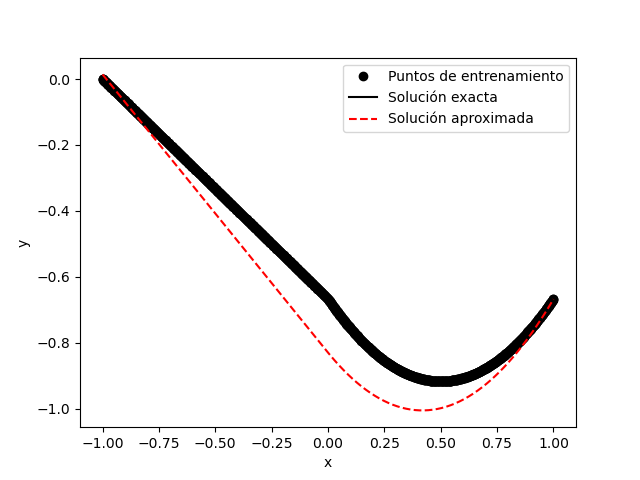
\includegraphics[width=0.6\textwidth]{Figuras/fallo_edp_pinn.png}
            \caption{Solución de la ecuación}
            \label{fig:deviation}
        \end{figure}

        Obviamente, el método no logra encontrar la solución exacta $u$. La diferencia entre $u$ y $\hat{u}(\mathbf{x};\theta)$ es tan grande como la magnitud de $u$, es decir, cuanto más grande es la solución en valor absoluto, nuestra aproximación se aleja más de ella. Además, si nos fijamos en la gráfica de entrenamiento y test, vemos que el error relativo a la solución real, calculado con la distancia de $L_2$ no disminuye con el número de iteraciones.
        \begin{figure}[H]
            \centering
            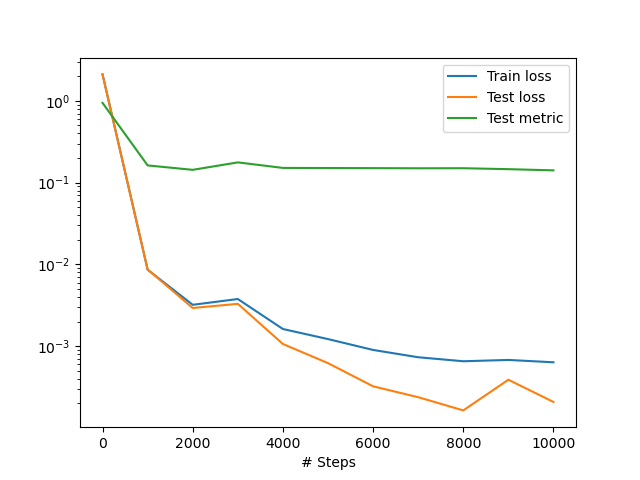
\includegraphics[width=0.6\textwidth]{Figuras/test_train_pinn_error.png}
            \caption{Error de la red neuronal}
        \end{figure}

        En esta gráfica, las curvas \textit{Error entrenamiento} y \textit{Error test} hacen referencia al error de la aproximación en los puntos de entrenamiento y test respectivamente. Por otro lado, el error relativo L2 mide la diferencia entre la función aproximada por la red neuronal y la solución real, evaluando dicha diferencia mediante su integración sobre el dominio, $(-1,1)$ en este caso.

    \end{exmp}
\end{mdframed}

Como hemos visto, las PINN presentan errores significativos en ciertos problemas, lo que puede atribuirse a diversos factores. Uno de los principales desafíos de las PINN es la falta de garantía de unicidad en la solución. A diferencia de los métodos numéricos tradicionales, las PINN resuelven problemas de optimización no convexos, los cuales, por naturaleza, no aseguran una solución única. Esto implica que la red neuronal no tiene garantía de converger a la solución correcta y, de hecho, en muchos casos no lo hace. Es más, al igual que ocurre con otros algoritmos de inteligencia artificial, la red puede converger con la misma certeza (o error) hacia una solución incorrecta que hacia la solución real.

Otro obstáculo importante es la ausencia de una justificación teórica que determine cuáles son los hiperparámetros óptimos. Este problema añade incertidumbre al proceso de ajuste de la red, lo que complica la obtención de resultados precisos. Finalmente, otro aspecto problemático de las PINN es que aproximan el residuo de forma fuerte. Esto significa que, si no existe una solución en el sentido fuerte (como ocurre en algunos casos), la red neuronal no puede aproximar de forma adecuada la solución débil.

De estos problemas, los dos primeros son característicos del uso de redes neuronales, mientras que el tercero es específico del método. Con esto en mente, exploraremos un enfoque alternativo que considere la forma débil en la composición del residuo, lo que podría permitir superar esta limitación.


\section{El ``Deep Ritz Method''} \label{sec:DeepRitz}

El método ``Deep Ritz'' es una técnica numérica basada en las redes neuronales, que busca encontrar una solución a una ecuación en derivadas parciales utilizando su forma débil. Este método es más coherente con la formulación matemática del problema, y evita las restricciones demasiado fuertes que presentan las PINN. Para poder plantar el método, es necesario primero describir los problemas elípticos autoadjuntos.

\subsection{El problema elíptico autoadjunto}\label{sec:ProblemaAutoadjunto}

El problema elíptico autoadjunto  permite caracterizar las soluciones de las EDP elípticas como el mínimo de un funcional. Esto conecta de manera lógica con el enfoque de redes neuronales para aproximar soluciones, donde la función de coste de la red neuronal se puede definir como esta función. Al minimizarla, se obtiene una solución aproximada del problema original. No obstante, esto lo veremos más adelante en detalle. De momento, consideramos una EDP de la forma vista en la Sección \ref{sec:EDPs}, es decir, una EDP elíptica sujeta a condiciones de contorno Dirichlet:
\begin{equation} 
    \begin{cases} -\sum_{i,j=1}^{n} \frac{\partial}{\partial x_j}\left( a_{ij}(\mathbf{x})\frac{\partial u}{\partial x_i}\right) + \sum_{i=1}^{n} b_i(\mathbf{x})\frac{\partial u}{\partial x_i} + c(\mathbf{x})u = f(\mathbf{x}), &\qquad \mathbf{x}\in\Omega,\\ u(\mathbf{x}) = g(\mathbf{x}), &\qquad \mathbf{x}\in\partial\Omega. 
    \end{cases} 
\end{equation} 
Así, se define el problema elíptico autoadjunto de la siguiente forma.
\begin{mdframed}
\begin{defin}
    Dado un conjunto $\Omega$, acotado y abierto en $\mathbb{R}^n$, decimos que una ecuación en derivadas parciales elíptica es autoadjunta,si se cumplen las siguientes condiciones de simetría en los coeficientes.
    \begin{equation}\label{eq:simetria_a}
        \begin{split}
            a_{ij} = a_{ji},\qquad &i,j = 1,\dots,n,\\
            b_i = 0, \qquad &i = 1,\dots,n,
        \end{split}
    \end{equation}
\end{defin}
\end{mdframed}
Bajo estas condiciones, nuestro problema se puede formular de la siguiente forma.
\begin{equation} \label{eq:ProblemaAutoadjuntoFuerte}
    \begin{cases}
        -\sum_{i,j=1}^{n} \frac{\partial}{\partial x_j}\left( a_{ij}(x)\frac{\partial u}{\partial x_i}\right) + c(x)u = f(x), & x\in\Omega,\\
        u(x) = 0, & x\in\partial\Omega.
    \end{cases}
\end{equation}

Por lo visto en la Sección \ref{sec:EDPs}, el problema \eqref{eq:ProblemaAutoadjuntoFuerte} se puede reescribir en forma débil de la siguiente forma: encontrar $u\in H_0^1(\Omega)$ tal que
\begin{equation}\label{eq:ProblemaAutoadjuntoDebil}
    a(u,v) = l(v) \quad \forall v\in  H_0^1(\Omega).
\end{equation}
Donde, al ser un problema autoadjunto, el funcional $a(\cdot,\cdot)$ es simétrico
\begin{equation*}
    a(u,w) = a(w,u) \quad \forall u,w\in H_0^1(\Omega).
\end{equation*}

De ahora en adelante vamos a asumir que \eqref{eq:ProblemaAutoadjuntoFuerte} cumple las condiciones de elipticidad uniforme y además se cumple que
\begin{equation*}
    c(x) - \frac{1}{2} \sum_{i=1}^n \frac{\partial b_i}{\partial x_i} \geq 0, \quad x \in \overline{\Omega},
\end{equation*}
por lo que, tal como se estableció en la sección \ref{sec:EDPs}, el problema \eqref{eq:ProblemaAutoadjuntoFuerte} admite una única solución débil. En consecuencia, si se satisfacen las condiciones correspondientes, la solución débil de \eqref{eq:ProblemaAutoadjuntoDebil} no solo es única, sino que también puede caracterizarse como el mínimo de un funcional. Esto es así por el siguiente resultado.



\begin{lema} \label{lema:MinimoFuncion}
    
    Definimos el funcional cuadrático $J: H_0^1(\Omega) \to \mathbb{R}$ como
    \begin{equation*}
        J(u) = \frac{1}{2}a(v,v) - l(v), \quad u\in H_0^1(\Omega),
    \end{equation*}
    de modo que las siguientes afirmaciones son equivalentes:
    \begin{enumerate}
        \item Encontrar el único $u\in H_0^1(\Omega)$ tal que $a(u,v) = l(v) \quad \forall v\in H_0^1(\Omega)$
        \item Encontrar el único $u\in H_0^1(\Omega)$ tal que $J(u) \leq J(v) \quad \forall v\in H_0^1(\Omega)$
    \end{enumerate}
\end{lema}
\begin{dem}
    ÁQUÍ PORÍA IR LA DEMOSTRACIÓN
\end{dem}

\subsection{Formulación del método ``Deep Ritz''}

ESTO ESTÁ BASTANTE CALCADO DEL PAPER A FALTA DE ACLARAR ALGUNOS CONCEPTOS

El método ``Deep Ritz'' busca resolver problemas de la siguiente forma:

\colorbox{yellow}{ESTO ME CHIRRÍA, VOY A DEJAR LA NOTACIÓN DEL}

\colorbox{yellow}{PAPER, PERO NO VEO MUY BIEN COMO CASA CON EL FUNCIONAL J}

\begin{equation}
\min_{u \in H} I(u)
\end{equation}
donde
\begin{equation}
I(u) = \int_{\Omega} \left( \frac 12  |\nabla u(x)|^2 -  f(x) u(x) \right) dx
\label{I(u)}
\end{equation}
y $H$ es el conjunto de funciones admisibles (también llamado función de prueba, representada aquí por $u$), $f$ es una función dada, que representa la fuerza externa aplicada al sistema en consideración. Problemas de este tipo son bastante comunes en las ciencias físicas. El método Deep Ritz se basa en el siguiente conjunto de ideas:

\begin{enumerate}
\item Aproximación basada en redes neuronales profundas para la función de prueba.
\item Una regla de cuadratura numérica para el funcional.
\item Un algoritmo para resolver el problema de optimización final.
\end{enumerate}


El componente básico del método Deep Ritz es una transformación no lineal $ x \rightarrow z_\theta (x)\in \mathbb{R}^{m} $ definida por una red neuronal profunda. Aquí $\theta$ denota los parámetros, típicamente los pesos de la red neuronal, que ayudan a definir esta transformación. En la arquitectura que utilizamos, cada capa de la red se construye apilando varios bloques, cada bloque consiste en dos transformaciones lineales, dos funciones de activación y una conexión residual. Tanto la entrada $s$ como la salida $t$ del bloque son vectores en $\mathbb{R}^{m}$. El $i$-ésimo bloque puede expresarse como:
\begin{equation}
t=f_i(s)=\phi(W_{i,2} \cdot \phi(W_{i,1} s +b_{i,1})+b_{i,2})+s
\label{block}
\end{equation}
donde $W_{i,1},W_{i,2} \in \mathbb{R}^{m \times m}$, $b_{i,1},b_{i,2} \in \mathbb{R}^{m}$ las correspondientes matrices de pesos y sesgos asociadas al bloque $i$. $\phi$ es la función de activación (escalar)

Tal y como se precisa en \cite{e2017deepritzmethoddeep} la función de activación $\phi$ juega un papel clave en la precisión del algoritmo. Para equilibrar simplicidad y precisión, hemos decidido utilizar 
\begin{equation}
\phi(x)=\max\{x^3,0\}
\end{equation}
El último término en \eqref{block}, la conexión residual, facilita mucho el entrenamiento de la red ya que ayuda a evitar el problema del gradiente que desaparece. La estructura de los dos bloques, incluyendo dos conexiones residuales, se muestra en la Figura \ref{fig:net_structure_1}.
 
\begin{figure}[!h]
\centering
\vspace{2pt}
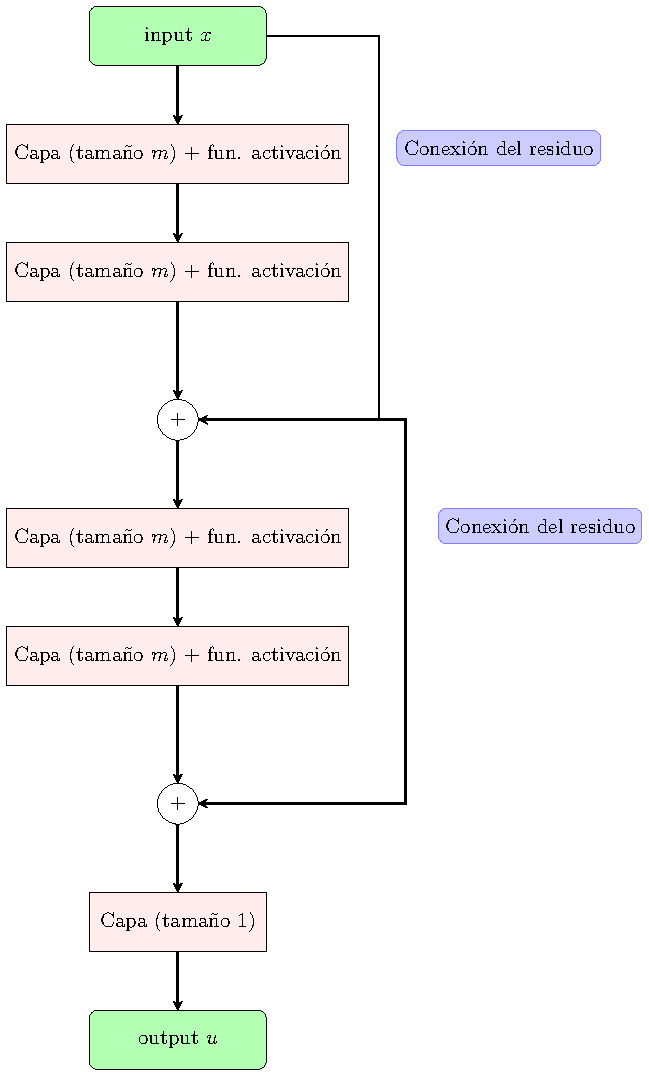
\includegraphics[width=0.5\textwidth]{TEX_Figures/deep_ritz_nn.pdf}
\caption{La figura muestra una red con dos bloques y una capa lineal de salida.
Cada bloque consiste en dos capas completamente conectadas y una conexión de salto.\label{fig:net_structure_1}}
\end{figure}

La red completa de $n$ capas puede expresarse ahora como:
\begin{equation}
z_{\theta}(x)=f_n\circ ... \circ f_1(x)
\end{equation}
$\theta$ denota el conjunto de todos los parámetros en toda la red.
Nota que la entrada $x$ para el primer bloque está en $\mathbb{R}^d$, no en $\mathbb{R}^{m}$.
Para manejar esta discrepancia podemos ya sea
completar $x$ con un vector de ceros cuando $d<m$, o aplicar una transformación lineal 
a $x$ cuando $d>m$. 
Teniendo $z_\theta$, obtenemos $u$ mediante
\begin{equation}
u(x; \theta) = a \cdot z_\theta (x) + b
\label{function-form}
\end{equation}
Aquí en el lado izquierdo y en lo que sigue, usaremos
$\theta$ para denotar el conjunto completo de parámetros $\{\theta, a, b \}$. Sustituyendo esto en la forma de $I$, obtenemos una función de $\theta$,
que debemos minimizar.

Para el funcional que aparece en \eqref{I(u)}, denotamos:
\begin{equation}
g(x; \theta) = \frac 12 |\nabla_x u(x; \theta)|^2 - f(x) u(x; \theta)
\end{equation}
entonces nos queda el problema de optimización:
\begin{equation}
\min_\theta L(\theta), \quad L(\theta) = \int_\Omega g(x; \theta) dx
\label{integral}
\end{equation}

El cual, de nuevo se resuelve mediante algoritmos de optimización basados en gradientes.

Al igual que hicimos en la sección \ref{sec:PINN}, vamos a ver dos ejemplos de la aplicación de las PINN a problemas concretos. 
\begin{mdframed}  
\begin{exmp}
    Consideremos el problema 
    
    \colorbox{yellow}{Esto solo esta transcrito, falta sacar conclusiones}
    \begin{equation*}
    -u'' = 1, \quad u(0) = u(1) = 0,
    \end{equation*}
    cuya solución exacta es 
    \begin{equation*}
    u(x) = -x^2/2 + x/2.
    \end{equation*}
    Planteamos el método de Ritz para este problema (\(f = 1\): \(\Omega = (0,1)\)),
    encontrar 
    \begin{align*}
    \min_{u_0} \left( \frac{1}{2} \int_\Omega \left((u_0')^2 - \int_\Omega fu_0 + \lambda (u_0(0)^2 + u_0(1)^2)\right)\right) =\\
    \min_{u_0} \left(\frac{1}{2} \int_0^1 \left((u_0')^2 - \int_0^1 fu_0 + \lambda (u_0(0)^2 + u_0(1)^2)\right)\right),
    \end{align*}
    donde \(u_0\) es una función de una red neuronal.
    Si consideramos el funcional \(J: H^1(0,1) \to \mathbb{R}\) definido por 
    \begin{equation*}
    J(u) = \frac{1}{2} \int_0^1 \left((u')^2 - \int_0^1 fu + \lambda (u(0)^2 + u(1)^2)\right)
    \end{equation*}
    y buscamos un mínimo, vamos a encontrar \(u\) tal que
    \begin{equation*}
    J'(u)v := \lim_{\beta \to 0} \frac{J(u + \beta v) - J(u)}{\beta} = 0.
    \end{equation*}
    Es fácil ver que \(u\) verifica, \(u \in H^1(0,1)\), y 
    \begin{equation*}
    \int_0^1 u'v' - \int_0^1 fv + 2\lambda u(0)v(0) + 2\lambda u(1)v(1) = 0, \quad \forall v \in H^1(0,1).
    \end{equation*}
    Consideramos ahora el siguiente problema: encontrar \(u \in C^2(0,1)\) tal que 
    \begin{equation*}
    -u'' = f, \quad u'(0) = 2\lambda u(0), \quad u'(1) = -2\lambda u(1),
    \end{equation*}
    que tiene como solución para \(f = 1\)
    \begin{equation*}
    u_\lambda = -x^2/2 + x/2 + 1/(4\lambda).
    \end{equation*}
    La solución débil de este problema es: encontrar \(u \in H^1(0,1)\) tal que 
    \begin{equation*}
    \int_0^1 u'v' + 2\lambda u(1)v(1) + 2\lambda u(0)v(0) = \int_0^1 fv, \quad \forall v \in H^1(0,1).
    \end{equation*}
    O lo que es lo mismo, encontrar \(u \in H^1(0,1)\) tal que 
    \begin{equation*}
    \int_0^1 u'v' + 2\lambda v(1)u(1) + 2\lambda v(0)u(0) = \int_0^1 fv, \quad \forall v \in H^1(0,1).
    \end{equation*}
\end{exmp}
\end{mdframed}

\chapter{Resultados}\label{chap3}

\chapter{Partes eliminadas - NO IMPRIMIR}
\section{Espacios de funciones}

Para poder entender y formular de forma matemática el problema de aproximación de EDPs mediante redes neuronales, es necesario tener un conocimiento previo de los espacios de funciones en los que trabajamos. Como veremos más adelante al estudiar los problemas de frontera para EDPs elípticas, es importante tener una caracterización del espacio $H_1^0$. Para entenderlo, empezaremos por los espacios de Hilbert Soobolev.

\begin{mdframed}
\begin{defin}
    Seam $\Omega$ un conjunto abierto de $\mathbb{R}^n$. Definimos el espacio de Sobolev $H^1(\Omega)$ como el conjunto de funciones en el siguiente conjunto
    \begin{equation}
        H^1(\Omega)=\{u\in L^2(\Omega): \frac{\partial u}{\partial x_i}\in L^2(\Omega), \, i=1,\dots,n\}.
    \end{equation}
    En este espacio, se define la norma de funciones de con la siguiente ecuación
    \begin{equation}
        \|u\|_{H^1(\Omega)}=\left(\|u\|^2_{L^2(\Omega)} + \sum_{i=1}^{n}\left\|\frac{\partial u}{\partial x_i}\right\|^2_{L^2(\Omega)}\right)^{1/2}.
    \end{equation}
\end{defin}
\end{mdframed}

Dada esta definición, se define el espacio $H_0^1(\Omega)$ como el cierre de las funciones de $C_0^\infty(\Omega)$ en la norma de $H^1(\Omega)$. Es decir, $H_0^1(\Omega)$ es el conjunto de funciones $u\in H^1(\Omega)$ que se obtienen como límite en $H^1(\Omega)$ de una serie de funciones $\{u_m\}_{m=1}^\infty$ todas ellas en $C_0^\infty(\Omega)$. Así, de forma más simple, se puede demostrar que $H_0^1(\Omega)$ se trata del siguiente conjunto.

\begin{equation}
    H_0^1(\Omega)=\{u\in H^1(\Omega): u=0 \text{ en } \partial\Omega\}.
\end{equation}

Nótese que $H_0^1(\Omega)$ es un espacio de Hilbert con la misma norma y producto interno que $H^1(\Omega)$.



\begin{exmp}
    Es fácil ver por ejemplo que la función $u = x^2 + y^2 - 4$ pertenece a $H^1_0(C)$, siendo $C = \{(x,y)\in \mathbb{R}^2: x^2 + y^2 < 4\}$ el círculo abierto de radio 2 centrada en el origen. Esto se debe a que $u\in L^2(C)$ y además:
    \begin{equation*}
        \frac{\partial u}{\partial x} = 2x\in L^2(C), \quad \frac{\partial u}{\partial y} = 2y \in L^2(C), \quad u=0\text{ en  } \partial C.
    \end{equation*}
    Por tanto, $u\in H_0^1(C)$.
\end{exmp}


\section{Introducción a las ecuaciones en derivadas parciales}

Las ecuaciones en derivadas parciales (EDPs) son ecuaciones que relacionan una función desconocida con sus derivadas parciales. Son fundamentales en la física y en la ingeniería, ya que permiten modelar fenómenos físicos y predecir su evolución en el tiempo. 

Existen varios tipos de EDPs, no obstante, nosotros nos centraremos en los problemas de frontera para ecuaciones en derivadas parciales elípticas. Estas se utilizan para resolver problemas de equilibrio, que implican encontrar la solución de una ecuación diferencial en un dominio acotado con condiciones de frontera específicas. Estos problemas incluyen la distribución estacionaria de temperatura, el flujo de fluidos incompresibles no viscosos, la distribución de tensiones en sólidos en equilibrio, y el cálculo de campos eléctricos en regiones con densidad de carga. En general, se aplican cuando se busca determinar un potencial en situaciones estacionarias. 

Lo he sacado de: \href{https://www.ugr.es/~prodelas/ftp/ETSICCP/Resoluci%F3nNum%E9ricaEDPs.pdf}{este enlace, \colorbox{yellow}{este tipo de cosas se citan?}}


%se puede hablar de los espacios de funciones en los que trabajamos, que es el supp de una función. Poner un ejemplo de ecuación diferencial y por que no se puede encontrar su solución en forma fuerte
Uno de los primero ejemplos de este tipo de ecuaciones es la ecuación de Poisson,
\begin{equation*}
    -\Delta  u = f,
\end{equation*}
donde $\Delta$ es el operador laplaciano, que se define como la suma de las segundas derivadas parciales de la función $u$:
\begin{equation*}
    \Delta u = \sum_{i=1}^{n}\frac{\partial^2 u}{\partial x_i^2}
\end{equation*}

Esta ecuación es una EDP elíptica pues cumple la siguiente definición general.


\begin{mdframed}
\begin{defin}
    Dado un conjunto $\Omega$, acotado y abierto en $\mathbb{R}^n$, decimos que una ecuación en derivadas parciales es elíptica si:
    \begin{equation}
        -\sum_{i,j=1}^{n} \frac{\partial}{\partial x_j}\left( a_{ij}(x)\frac{\partial u}{\partial x_i}\right) + \sum_{i=1}^{n} b_i(x)\frac{\partial u}{\partial x_i} + c(x)u = f(x), \qquad x\in\Omega.
    \end{equation}
    Donde los coeficientes $a_{ij}(x)$, $b_i(x)$, $c(x)$ y $f$ son funciones que satisfacen las siguientes condiciones
    \begin{align}
        a_{ij} \in C^1(\overline{\Omega}),& \qquad i,j = 1, \dots ,n \\
        b_i, c \in C(\overline{\Omega}),& \qquad i = 1, \dots ,n \\
        c \in C(\overline{\Omega}),& \\
        f\in C(\overline{\Omega})&
    \end{align}
\end{defin}
\end{mdframed}

De entre los problemas elípticos definidos en \ref{def:EDP_eliptica}, como comentábamos, nos interesan las ecuaciones en derivadas parciales elípticas con condiciones de frontera, en concreto, las condiciones de frontera de Dirichlet.

\begin{mdframed}
\begin{defin}    
    El problema de condición de frontera de Dirichlet es concretamente el que tenemos una EDP elíptica como la definida en \ref{def:EDP_eliptica}, tal que, nuestra solución $u$, además de cumplir las ecuación \eqref{eq:EDP_eliptica}, cumple la siguiente condición de frontera
    \begin{equation}
        u(x) = g(x), \qquad \forall x\in\partial\Omega.
    \end{equation}
    Asimismo, el problema homogéneo de Dirichlet es aquel en el que $g=0$. A lo largo del trabajo nos centraremos principalmente en es te tipo de EDPs.
\end{defin}
\end{mdframed}

Con todo, el tipo de ecuaciones elípticas en el que nos vamos a centrar (entendiendo que se cumplen las condiciones de \eqref{eq:condiciones_EDP_eliptica_a} - \eqref{eq:condiciones_EDP_eliptica_f}) serán de la siguiente forma.
\begin{equation}
    \begin{cases}
        -\sum_{i,j=1}^{n} \frac{\partial}{\partial x_j}\left( a_{ij}(x)\frac{\partial u}{\partial x_i}\right) + \sum_{i=1}^{n} b_i(x)\frac{\partial u}{\partial x_i} + c(x)u = f(x), \qquad & x\in\Omega \\
        u(x) = 0, & x\in\partial\Omega.
    \end{cases}
\end{equation}

\section{Forma fuerte y débil de una EDP}
En la formulación que hemos dado de las ecuaciones en derivadas parciales elípticas, nos estábamos refiriendo a su formulación en forma fuerte. De forma intuitiva, esta es la que se obtiene directamente de la definición de la ecuación, y es la que relaciona la función desconocida con sus derivadas parciales. La solución de estas ecuaciones en forma fuerte es la que se conoce como solución clásica. De esto surge la siguiente definición.

\begin{mdframed}
\begin{defin}
    Una función $u \in C^2(\Omega)$ que cumples las condiciones de frontera de Dirichlet y satisface la ecuación \eqref{eq:EDP_eliptica} en $\Omega$ se dice que es una solución clásica o fuerte de la ecuación \eqref{eq:EDP_eliptica}. 
\end{defin}
\end{mdframed}

No obstante, en muchos casos, no es posible encontrar una solución en forma fuerte, es decir, una función que cumpla la ecuación en todo el dominio y que además cumpla las condiciones de frontera. En estos casos, se recurre a métodos alternativos, como la formulación débil de la ecuación, que permite encontrar una solución en un espacio de funciones más amplio. A continuación, vemos un ejemplo que motiva la necesidad de recurrir a la formulación débil de una ecuación.

\begin{exmp}
    Supongamos que tenemos la siguiente ecuación de Poisson con una condición de frontera de Dirichlet homogénea,
    \begin{equation*}
        \begin{cases}
            -\Delta u = f, & \text{en } \Omega,
            \\
            u = 0, & \text{en } \partial\Omega.
        \end{cases}
    \end{equation*}
    Donde $\Omega$ es un conjunto acotado y abierto en $\mathbb{R}^n$. En este caso, no siempre es posible encontrar una solución en forma fuerte, es decir, una función $u$ que cumpla la ecuación en todo el dominio $\Omega$ y que además cumpla la condición de frontera. Por ejemplo, si $f$ no es una función suave, no se puede garantizar la existencia de una solución en forma fuerte pues estaríamos rompiendo la condición de \eqref{eq:condiciones_EDP_eliptica_f}. En estos casos, se recurre a métodos alternativos, como la formulación débil de la ecuación, que permite encontrar una solución en un espacio de funciones más amplio. 
\end{exmp}


Para pasar de forma fuerte a débil, lo que hacemos es seguir el siguiente proceso
\begin{enumerate}
    \item Multiplicamos a ambos lados de la igualdad por una función $\varphi \in C^\infty_0(\Omega)$ e integramos.
    \begin{align*}
        \int_\Omega\left(-\sum_{i,j=1}^{n} \frac{\partial}{\partial x_j}\left( a_{ij}(x)\frac{\partial u}{\partial x_i}\right) + \sum_{i=1}^{n} b_i(x)\frac{\partial u}{\partial x_i} + c(x)u \right) \varphi  \,dx\\ =\int_\Omega f(x)\varphi  \,dx
    \end{align*}
    \item Expandimos la multiplicación e integramos por partes en la primera integral, llegando a
    \begin{align*}
        \sum_{i,j=1}^{n} \int_\Omega a_{ij}(x) \frac{\partial \varphi }{\partial x_j} \frac{\partial u}{\partial x_i} + \sum_{i=1}^{n} \int_\Omega b_i(x)\frac{\partial u}{\partial x_i}\varphi  + \int_\Omega c(x)\varphi u  \,dx\\ =\int_\Omega f(x)\varphi  \,dx
    \end{align*}
    Con esta manipulación hemos conseguido una cosa muy interesante: ya no tenemos segundas derivadas de $u$, es decir, ya no necesitamos que $u\in C^2$. Para que esta igualdad tenga sentido, solo hace falta que $u\in L^2(\Omega)$ y que $\partial y /\partial x_i \in L^2(\Omega),\, i =1,\dots,n$. Nótese además que, para que se cumpla la condición de frontera de Dirichlet, $u=0 \in \partial\Omega$. Todo esto se traduce a que $u\in H_0^1(\Omega)$ Esto simplifica las condiciones del problema pues el espacio de funciones en el que puede estar $u$, ahora es mucho más amplio.
    \item Para simplificar aun más el problema, nótese que $a_{ij}$ ya no aparecen tras derivadas de ningun tipo, luego no es necesario asumir que $a_{ij}\in C^1(\overline{\Omega})$, basta con que $a_{ij}\in L^\infty(\Omega)$. Por lo mismo, $b_i,\,c\in L^\infty(\Omega), i=1,\dots,n$ es suficiente.
    \item Por último, nótese que $C^\infty_0(\Omega) \subset H^1_0(\Omega)$, luego se puede ver que teniendo $u,v\in H^1_0(\Omega)$, nuestra ecuación sigue teniendo sentido. Con todo esto, surge la siguiente definición de forma débil.
\end{enumerate}

\begin{mdframed}
    \begin{exmp}
        
        Resolveremos una ecuación de calor:
        \begin{equation*}
        \frac{\partial u}{\partial t} = \alpha \frac{\partial^2 u}{\partial x^2}, \quad x \in [0, 1], \quad t \in [0, 1]
        \end{equation*}
        donde \(\alpha = 0.4\) es la constante de difusividad térmica. Con condiciones de frontera de Dirichlet:
        \begin{equation*}
        u(0, t) = u(1, t) = 0,
        \end{equation*}
        y condición inicial periódica (sinusoidal):
        \begin{equation*}
        u(x, 0) = \sin\left(\frac{n \pi x}{L}\right), \quad 0 < x < L, \quad n = 1, 2, \ldots
        \end{equation*}
        donde \(L = 1\) es la longitud de la barra y \(n = 1\) es la frecuencia de la condición inicial sinusoidal.
        Para este problema, sabemos que la solución exacta es:
        \begin{equation*}
        u(x, t) = e^{-\frac{n^2 \pi^2 \alpha t}{L^2}} \sin\left(\frac{n \pi x}{L}\right).
        \end{equation*}
        Que si la vemos de forma gráfica, obtenemos la Figura \ref{fig:calor_exacta}.
        \begin{figure}[H] 
            \centering
            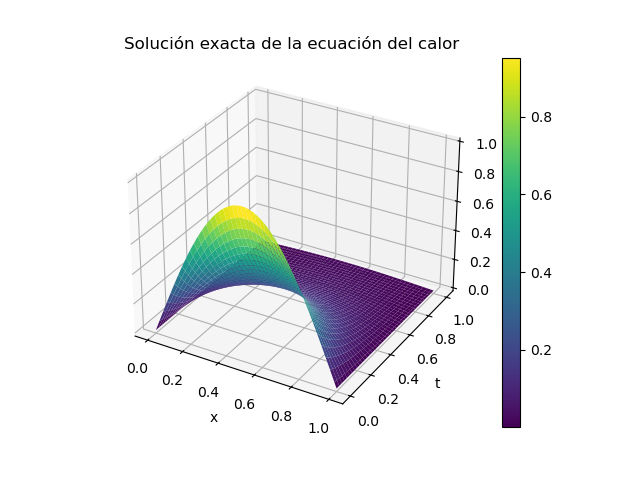
\includegraphics[width=0.5\textwidth]{Figuras/calor_exacta.png}
            \caption{Solución de la ecuación de calor}
            \label{fig:calor_exacta}
        \end{figure}
        Si nos ayudamos de la librería DeepXDE, podemos programar la red neuronal y entrenarla para que aproxime la solución de la ecuación de calor. El resultado obtenido es el obtenido en la Figura \ref{fig:calor_estimacion}.
        \begin{figure}[H] 
            \centering
            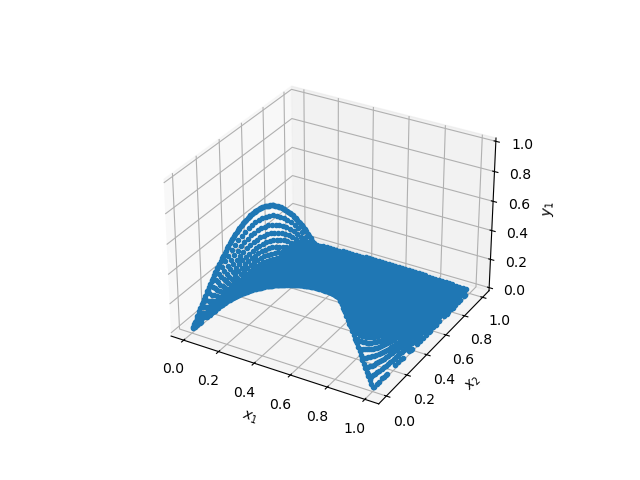
\includegraphics[width=0.5\textwidth]{Figuras/calor_estimacion.png}
            \caption{Aproximación de la solución de la ecuación de calor}
            \label{fig:calor_estimacion}
        \end{figure}

    \end{exmp}
\end{mdframed}

\begin{mdframed}
    \begin{exmp}
        Consideramos un problema de convección unidimensional, una EDP hiperbólica:
        \begin{equation*}
            \frac{\partial u}{\partial t} + \beta \frac{\partial u}{\partial x} = 0, \quad x \in \Omega, \; t \in [0, T],
        \end{equation*}
        \begin{equation*}
            u(x, 0) = h(x), \quad x \in \Omega.
        \end{equation*}
        Aquí, $\beta$ es el coeficiente de convección y $h(x)$ es la condición inicial. Para un $\beta$ constante y condiciones de contorno periódicas, este problema tiene una solución analítica simple:
        \begin{equation*}
            u_{\text{analytical}}(x, t) = \mathcal{F}^{-1} \big( \mathcal{F}(h(x)) e^{-i k \beta t} \big),
        \end{equation*}
        donde $\mathcal{F}$ es la transformada de Fourier, $i = \sqrt{-1}$ y $k$ denota la frecuencia en el dominio de Fourier. La función de pérdida general para este problema (correspondiente a la Ecuación \eqref{eq:L_PINN}) es
        \begin{equation*}
            \mathcal{L}(\theta) = \frac{1}{N_u} \sum_{i=1}^{N_u} \left( \hat{u} - u^0_i \right)^2 
            + \frac{1}{N_f} \sum_{i=1}^{N_f} \lambda_i \left( \frac{\partial \hat{u}}{\partial t} + \beta \frac{\partial \hat{u}}{\partial x} \right)^2 + \mathcal{L}_B,
        \end{equation*}
        donde $\hat{u}$ es la salida de la red neuronal, y $\mathcal{L}_B$ es la pérdida de contorno. Para condiciones de contorno periódicas con $\Omega = [0, 2\pi]$, esta pérdida es:
        \begin{equation*}
            \mathcal{L}_B = \frac{1}{N_B} \sum_{i=1}^{N_B} \left( \hat{u}(\theta, 0, t) - \hat{u}(\theta, 2\pi, t) \right)^2.
        \end{equation*}
        Usamos las siguientes condiciones iniciales y de contorno periódico simples:
        \begin{align*}
            u(x, 0) = \sin(x),\\
            u(0, t) = u(2\pi, t).
        \end{align*}
        Si usamos la librería propuesta por Xu et al. en el Repositorio \cite{c2021failure} para resolver este problema, obtenemos la aproximación se puede ver en la Figura \ref{fig:error_PINN_temporal}. En esta, se puede observar que la aproximación y la solución exacta no coinciden y además, el error es muy elevado para $\beta > 1$.
        \begin{figure}[H]
            \centering
            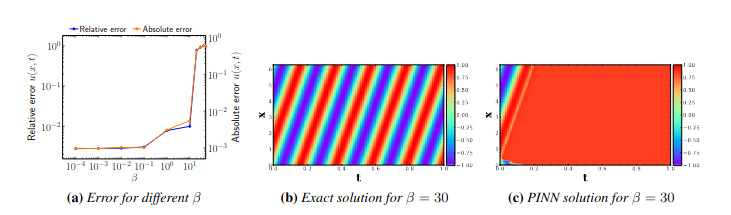
\includegraphics[width=0.9\textwidth]{Figuras/error_PINN_temporal.png}
            \caption{Solución de la ecuación de convección}
            \label{fig:error_PINN_temporal}
        \end{figure}

    \end{exmp}
\end{mdframed}

\printbibliography
\cleardoublepage


\end{document}
